\documentclass[preprint,12pt]{elsarticle}
%% Use the options 1p,twocolumn; 3p; 3p,twocolumn; 5p; or 5p,twocolumn
%% By default, use:
%% \documentclass[preprint,12pt]{elsarticle}
%% for a journal layout:
%% \documentclass[final,1p,times]{elsarticle}
%% \documentclass[final,1p,times,twocolumn]{elsarticle}
%% \documentclass[final,3p,times]{elsarticle}
%% \documentclass[final,3p,times,twocolumn]{elsarticle}
%% \documentclass[final,5p,times]{elsarticle}
%% \documentclass[final,5p,times,twocolumn]{elsarticle}

%% PREAMBLE =========================================
%\input{__sec_preamble}
% Input and font
\usepackage[utf8]{inputenc}
\usepackage[T1]{fontenc}
\usepackage{lmodern}
\usepackage[english]{babel}

% Page layout and spacing
%\usepackage[margin=2.5cm]{geometry}
%\usepackage{setspace}
%\onehalfspacing

% Math
\usepackage{amsmath, amssymb, amsfonts}
\usepackage{siunitx}

% Tables
\usepackage{booktabs}
\usepackage{multirow}
\usepackage{array}
\usepackage{tabularx}
\usepackage{longtable}
\sisetup{
    table-format = 1.6,
    round-mode = places,
    round-precision = 3,
    detect-mode,
    detect-family,
    detect-inline-family=math,
}
\sisetup{zero-decimal-to-integer}

% Graphics
\usepackage{graphicx}
\usepackage{float}
\usepackage{subfig}
\usepackage{caption}
\usepackage{subcaption}
\usepackage{todonotes}

% Colors
\usepackage{xcolor}

% Citations and references
\usepackage{natbib}
%\bibliographystyle{unsrtnat}

% Hyperlinks
\usepackage[colorlinks=true, linkcolor=blue, citecolor=blue, urlcolor=blue]{hyperref}

% Glossaries and acronyms
% \usepackage[acronym]{glossaries}
% \makeglossaries
\usepackage{acro}

% Cross-references
\usepackage{cleveref}

% Custom commands
\newcommand{\inserttable}[1]{\input{tables/#1}}
\newcommand{\insertfigure}[1]{\input{figures/#1}}

% Diagrams
\usepackage{tikz}
\usetikzlibrary{positioning, shapes, calc}

\journal{Results in Engineering}
%% END PREAMBLE ----------------------------------

% load acronyms from external file
\input{__sec_acronyms}

\begin{document}

\begin{frontmatter}

%% Title, authors and addresses

%% use the tnoteref command within \title for footnotes;
%% use the tnotetext command for theassociated footnote;
%% use the fnref command within \author or \affiliation for footnotes;
%% use the fntext command for theassociated footnote;
%% use the corref command within \author for corresponding author footnotes;
%% use the cortext command for theassociated footnote;
%% use the ead command for the email address,
%% and the form \ead[url] for the home page:
%% \title{Title\tnoteref{label1}}
%% \tnotetext[label1]{}
%% \author{Name\corref{cor1}\fnref{label2}}
%% \ead{email address}
%% \ead[url]{home page}
%% \fntext[label2]{}
%% \cortext[cor1]{}
%% \affiliation{organization={},
%%             addressline={},
%%             city={},
%%             postcode={},
%%             state={},
%%             country={}}
%% \fntext[label3]{}

\title{Lightweight Single-Cycle Prognostics for Li-ion Batteries: Feature Extraction and Cross-Cell Generalization}

%% use optional labels to link authors explicitly to addresses:
%% \author[label1,label2]{}
%% \affiliation[label1]{organization={},
%%             addressline={},
%%             city={},
%%             postcode={},
%%             state={},
%%             country={}}
%%
%% \affiliation[label2]{organization={},
%%             addressline={},
%%             city={},
%%             postcode={},
%%             state={},
%%             country={}}

%% Author affiliation
\affiliation[unicamp_feec]{
    organization={Faculty of Electrical and Computer Engineering (FEEC), State University of Campinas (UNICAMP)},%Department and Organization
        addressline={Albert Einstein Avenue, 400; Cidade Universitária}, 
        city={Campinas},
        postcode={13083-852}, 
        state={SP},
        country={Brazil}
}
\affiliation[thi_cecos]{
    organization={Research group “Safe Electromobility and Accident Analysis”, CARISSMA Institute for Electric, Connected and Safe Mobility (C-ECOS), Technische Hoschschule Ingolstadt (THI)},%Department and Organization
    addressline={Esplanade 10}, 
    city={Ingolstadt},
    postcode={85049}, 
    state={Bayern},
    country={Germany}}


%% Author name
\author[unicamp_feec]{Gabriel Buzzi Sanches} %\ead{g256389@dac.unicamp.br}
\author[unicamp_feec,thi_cecos]{Carlos Antônio Rufino Jr.\corref{cor1}} \ead{carlos.rufino@carissma.eu}
\author[unicamp_feec]{Lucas Saraiva Teixeira\corref{cor1}} \ead{lucas.sarvtex@gmail.com}
\author[thi_cecos]{Hans-Georg Schweiger}
\author[unicamp_feec]{Hudson Giovani Zanin\corref{cor1}} \ead{hzanin@unicamp.br}

\cortext[cor1]{Corresponding authors}



%% Abstract
\begin{abstract}
Accurate estimation of State of Health (SOH) and Remaining Useful Life (RUL) is critical for the reliability of Lithium-ion batteries. However, existing data-driven approaches often rely on computationally intensive deep learning architectures or require long, continuous degradation histories, limiting their deployment in embedded Battery Management Systems (BMS). This study proposes a lightweight, machine learning framework capable of robust prognostics using features extracted from a single diagnostic charge-discharge cycle for model inference. Utilizing a dataset of 124 commercial LFP/graphite cells cycled under fast-charging conditions, we extracted 16 statistical features from voltage, current, and temperature profiles. We evaluated four regression algorithms—including LightGBM and Extra Trees—optimized via Tree-structured Parzen Estimators (TPE). The proposed models demonstrated strong cross-cell generalization on unseen data, achieving a median Root Mean Squared Error (RMSE) of 0.71\% for SOH and approximately 60 cycles for RUL. Furthermore, feature importance analysis revealed that reducing the input space to just four key features maintained predictive accuracy, confirming the method's viability for resource-constrained, real-time applications.




%% Version 2
%Accurately estimating State of Health (SOH) and Remaining Useful Life (RUL) for Lithium-ion Batteries, an application very much suited for Machine Learning, is necessary for enabling advanced battery management and delivering a more predictable and reliable consumer product. However, given that batteries are a fast evolving technology, it can often be difficult to acquire the large, high-quality battery aging datasets needed to train such models. In these cases, good feature extraction -- making the most from the data in these datasets -- is essential. Using the public Severson dataset (124 LFP cells), this paper was successfully able to create lightweight Gradient Boosting and Random Forest Regressor models with median Root Mean Squared Errors (RMSE) ranging from 0.7--0.8 percentage points for SOH and 42--60 cycles for RUL by extracting 16 informative statistical features from single cycle Voltage, Current, and Temperature data. Our analysis highlights the most informative features, the trade-off between feature count and accuracy, and the deployment potential of lightweight models. Limitations include it being LFP only and relying on a special diagnostic cycle, which future work will address.

%% Text of abstract
% This paper proposes a single-cycle, feature-based approach for estimating the \acf{soh} and \acf{rul} of lithium-ion batteries. Using the public Severson LFP dataset (124 cells), we extract 16 statistical features from voltage, current, and temperature signals of a diagnostic full cycle. Gradient boosting and random forest regressors are trained with cell-wise cross-validation and tested on 25 unseen cells. Results show a median RMSE of 0.7--0.8\% for SoH~\cref{tab:soh_metrics} and 42--60 cycles for RUL~\cref{tab:rul_metrics}, with consistent generalization across batches. Our analysis highlights the most informative features, the trade-off between feature count and accuracy, and the deployment potential of lightweight models. Limitations include the single chemistry and the need for diagnostic cycles, which future work will address.
\end{abstract}

%%Graphical abstract
%\begin{graphicalabstract}
%\includegraphics{grabs}
%\end{graphicalabstract}

%%Research highlights
\begin{highlights}
\item The framework enables SOH and RUL inference on unseen battery cells using models trained on publicly available data, requiring only a single cycle from the target cell.
\item Robust cross-cell generalization is demonstrated on 124 LFP cells, achieving median RMSEs of 0.7-0.8\% for SOH and 42-60 cycles for RUL.
\item Feature selection reveals that reducing inputs from 16 to just 4 key variables maintains predictive accuracy while significantly lowering computational cost.
\item The use of lightweight decision-tree ensembles offers a computationally efficient alternative to deep learning for deployment in resource-constrained environments.
%\item Research highlight 1
%\item Research highlight 2
\end{highlights}

%% Keywords
\begin{keyword} % keywords here, in the form: keyword \sep keyword
Battery prognostics \sep State of Health \sep Remaining Useful Life \sep Feature Engineering \sep LFP Battery \sep Gradient Boosting

\end{keyword}

\end{frontmatter}




\section{Introduction} \label{sec:intro}

The transition to renewable energy and the rapid adoption of electric mobility have placed \acf{libs} at the center of modern energy storage technologies. Ensuring their safety, reliability, and economic viability requires accurate monitoring of degradation and forecasting of future performance, a field known as battery prognosis. Two key indicators are \acf{soh}, the capacity relative to a new cell, and \acf{rul}, the cycles until a predefined end-of-life. Reliable estimation of these metrics is critical for optimizing battery use, enabling predictive maintenance, and extending system lifetime in applications such as electric vehicles and stationary storage systems.  

Despite significant progress, existing methods for battery prognosis face important challenges. Many \acf{ml} approaches rely on handcrafted features extracted from full charge--discharge cycles, which restricts their applicability to controlled datasets where continuous cycling data are available. More advanced deep learning methods have been proposed to process raw electrochemical signals directly, thereby bypassing manual feature engineering \cite{Che2022, Lv2024}. However, these approaches introduce substantial computational demands and often lack interpretability, which limits their deployment in embedded battery management systems. Furthermore, most studies validate their methods on laboratory datasets collected under highly controlled conditions, often with aggressive fast-charging protocols and uniform cycling patterns \cite{Jafari2024, Liu2025}. Such protocols do not reflect the intermittent and partial cycling profiles seen in real-world applications, reducing the generalizability of the resulting models.  

Another key limitation is the reliance on multiple consecutive cycles to extract reliable prognostic features. Operational systems rarely provide uninterrupted sequences of complete charge--discharge cycles, making such requirements impractical. This highlights the need for models capable of producing robust SoH and RUL estimates from limited information, ideally from a single diagnostic cycle, without assuming continuous access to full degradation histories.

In this work, we address these challenges by developing tree-based machine learning models \todo[size=\tiny]{[R1] Explain why this decided to use tree-based models as opposed to Deep Learning.}: trained on a large, publicly available dataset of 124 commercial LiFePO\textsubscript{4}/graphite cells cycled under fast-charging conditions \cite{sev2019}. The decision to focus on tree-based models, as opposed to deep-learning, is justified due to the nature of the dataset being  considered: high dimension, structured, tabular datasets; these are conditions classical machine learning deals very well. Additionally, these models are typically simpler and more appropriate in edge-computing, where resources are more strained.   % LOOK INTO GERON

Unlike prior studies that depend on sequences of multiple cycles, our methodology demonstrates that accurate inference of both SoH and RUL can be achieved using only the information contained in a single conventional charge-discharge cycle. \todo[size=\tiny]{[R1] What is the reason to use single-cycle? Explain it in more depth.} This approach reflects a realistic diagnostic scenario where historical battery data is unavailable (thus the need of a single cycle) and without requiring normal operation to be interrupted and a specialized time-consuming diagnostic protocol to be performed (which explains the preference for operational data). By extracting statistical features from voltage, current, and temperature signals at the cycle level, we provide a compact and computationally efficient representation suitable for supervised learning. The main contributions are twofold:

\begin{enumerate}[i]
    \item We show that reliable prognosis does not require long degradation histories for inference, thereby increasing the applicability of ML methods in real-world battery management systems.
    \item We present a systematic evaluation of feature-based models for SoH and RUL estimation, highlighting the balance between interpretability, efficiency, and predictive performance.  
\end{enumerate}



The rest of this work is structured as such: Sections \ref{sec:related_works}, \ref{sec:dataset}, \ref{sec:soh_rul}, and \ref{sec:data_analysis} introduce the theoretical backing of the paper, they include a literature review, a definition and description of the problem and an introduction and exploration of the dataset used within this model, from Severson et al \cite{sev2019}. Sections \ref{sec:feature_extraction}, \ref{sec:ml_models} and \ref{sec:optimiation} includes the bulk of the methodology; this includes the process of data clean-up and feature extraction, the various types of tree-based models under consideration and the process of training and hyper-parameters optimization. Section \ref{sec:results} discusses the results and Section \ref{sec:conclusions} concludes with a discussion. Table  \ref{tab:Acronyms} is a glossary with a list of all the acronyms used in this work.

\begin{table}[]
    \centering
    \printacronyms[template=tabular, name=Glossary]
    \caption{List of Acronyms found in this work.}
    \label{tab:Acronyms}
\end{table}

% (i) , and (ii) we present a systematic evaluation of feature-based models for SoH and RUL estimation, highlighting the balance between interpretability, efficiency, and predictive performance.  



\input{__sec01_related_work}
\section{Dataset Description} \label{sec:dataset}

The Severson dataset, used in this study, was first shown in reference \cite{sev2019}. It comprises cycling data from 124 commercial lithium iron phosphate (LFP) / graphite batteries, these batteries, manufactured by A123 Systems (model APR18650M1A), have a nominal capacity of 1.1 Ah and a nominal voltage of 3.3 V. The original study aimed to optimize fast charging for lithium-ion batteries, with all batteries cycled to failure under various fast-charging conditions in a controlled environment \todo[size=\tiny]{[R2] The dataset only contains the data of LFP batteries under fast-charging conditions in the lab. Have you considered the generalizatoin for other chemistries like NMC, NCA.}. In this work, the dataset was accessed using the provided MATLAB struct (\texttt{.mat}) files, which serve as a convenient container for individual cycle data and can be either by MATLAB or Python (via the h5py package). Pandas dataframes can also be generated from these structs using provided code.

The batteries were cycled in horizontal cylindrical fixtures on a 48-channel Arbin LBT potentiostat within a forced convection temperature chamber maintained at 30°C. Charging was performed using either one-step or two-step fast-charging policies, denoted as "C1(Q1)-C2," where C1 and C2 represent the constant current rates for the first and second steps, respectively, and Q1 indicates the state-of-charge (SOC, in \%) at which the current switches. The second current step concluded at 80\% SOC, followed by a 1C constant current-constant voltage (CC-CV) charging protocol. The upper and lower voltage cutoffs were selected in adherence with manufacturer specifications: at 3.6 V for maximum and 2.0 V for minimum. These voltage limits were enforced across all charging steps, including fast charging. In some cases, in sufficiently aged batteries, the upper voltage limit was reached during the fast charging phase, before reaching 80 SOC\%, which caused extended in extended constant-voltage charging periods when it occured. All batteries were discharged at a constant current rate of 4C.

The Severson dataset includes voltage, current, temperature, charge capacity, discharge capacity, and internal resistance measurements, for each cell and for each cycle. The temperature data was collected by attaching type T thermocouples to the exposed cell cans with thermal epoxy (OMEGATHERM 201) and Kapton tape, after removing a small section of the plastic insulation. However, the reliability of temperature measurements may vary due to inconsistent thermal contact between the thermocouple and the battery can, with some thermocouples losing contact during cycling. Internal resistance was measured during charging at 80\% SOC by averaging 10 pulses of ±3.6C, with a pulse width of 30 ms for Batches 1 and 2, or 33 ms for Batch 3. A summary of batches and charge/discharge protocols is shown in Table \ref{tab:batch_summary}.

% Batch summary
\begin{table}[ht]
\centering
\caption{Summary of Severson dataset batches and protocols.}
\label{tab:batch_summary}
\resizebox{\textwidth}{!}{%
\begin{tabular}{llll}
\hline
Batch & Charge protocol (CCCV) & Discharge protocol (CC) & Notes \\
\hline
1 & Variable C-rate, cutoff 3.6V & 4C to 2.0V & 45 cells, thermocouples present \\
2 & Variable C-rate, cutoff 3.6V & 4C to 2.0V & 43 cells, restart artifact \\
3 & Variable C-rate, cutoff 3.6V & 4C to 2.0V & 36 cells, longer rests \\

%1 & CCCV @ 1.5C (cutoff 3.6V) & CC 4C to 2.0V & 45 cells, thermocouples present \\
%2 & CCCV @ 1.5C (cutoff 3.6V) & CC 4C to 2.0V & 43 cells, restart artifact \\
%3 & CCCV @ 1.5C (cutoff 3.6V) & CC 4C to 2.0V & 36 cells, longer rests \\
\hline
\end{tabular}
}
\end{table}

% \insertfigure{fig_model}
% \inserttable{tbl_dataset}

\section{\acl{soh} and \acl{rul}} \label{sec:soh_rul}

The development of machine learning models for battery prognosis requires clearly defined target variables, namely \acf{soh} and \acf{rul} These metrics serve as key performance indicators to quantify the degradation state of a battery. The following section outlines the methodology used to calculate these ground-truth labels from the experimental cycling data.

The \acf{soh} of a battery provides a snapshot of its current condition relative to its initial, "healthy" state. It is typically expressed as a percentage of the nominal capacity. For the purpose of this study, the \ac{soh} for the nth cycle, denoted as $SoH_n$, is calculated as the ratio of the maximum discharge capacity observed during that cycle to the rated cell capacity, as shown in Equation \ref{eq:soh}.

\begin{equation}
    \mathrm{SoH}_n = \frac{Q_n}{Q_{\text{rated}}}
    \label{eq:soh}
\end{equation}

where $Q_n$ is the maximum discharge capacity recorded for the $n^{th}$ cycle, and $Q_{rated}$ is the rated capacity of a new cell.

A critical limitation in determining the ground-truth \ac{soh} in real-world applications is that batteries rarely undergo a full charge or discharge cycle. This makes it challenging to accurately measure the true capacity at any given time. The controlled laboratory setting used to generate this dataset, where full cycles are performed, provides a consistent and reliable method for calculating this critical ground truth.

The \ac{rul} of a battery represents the number of cycles it can endure before reaching its \ac{eol} condition. The \ac{eol} is a predefined failure threshold, commonly set when the battery's capacity drops to 80\% of its initial rated capacity. The \ac{eol} cycle is therefore defined as the cycle number at which the \ac{soh} first falls to 80\% or below.

\begin{equation}
    \mathrm{EoL} = \min \left\{ n \;\middle|\; \mathrm{SoH}_n \leq 0.80 \right\}
    \label{eq:eol}
\end{equation}

The \ac{rul} for any given cycle n, denoted as $\mathrm{RUL}_n$, is then calculated by subtracting the current cycle number from the \ac{eol} cycle number, as expressed in \cref{eq:rul} below.

\begin{equation}
    \mathrm{RUL}_n = \mathrm{EoL} - n
    \label{eq:rul}
\end{equation}

A significant challenge associated with using cycle count to define \ac{rul} is its limited applicability to real-world scenarios. In our dataset, cycles are a consistent, predictable, and well defined quantity; realistic use-cases often involve irregular charging and discharging patterns, which makes ``cycles'' an unreliable metric. Furthermore, determining the ground truth \ac{rul} for a particular cycle requires having the full degradation data up to the battery's \ac{eol}, which is a common limitation when training \ac{rul} prediction models from incomplete datasets.

Figure \ref{fig:targets_distribution} shows the distribution of both \ac{soh} and \ac{rul} on the Severson dataset \cite{sev2019}. Notably, neither target exhibits a symmetric distribution. The skewed nature  of require a machine learning model that is robust to non-normal data distributions and can effectively capture the non-linear degradation behavior of batteries.


\begin{figure}[H]
    \centering
    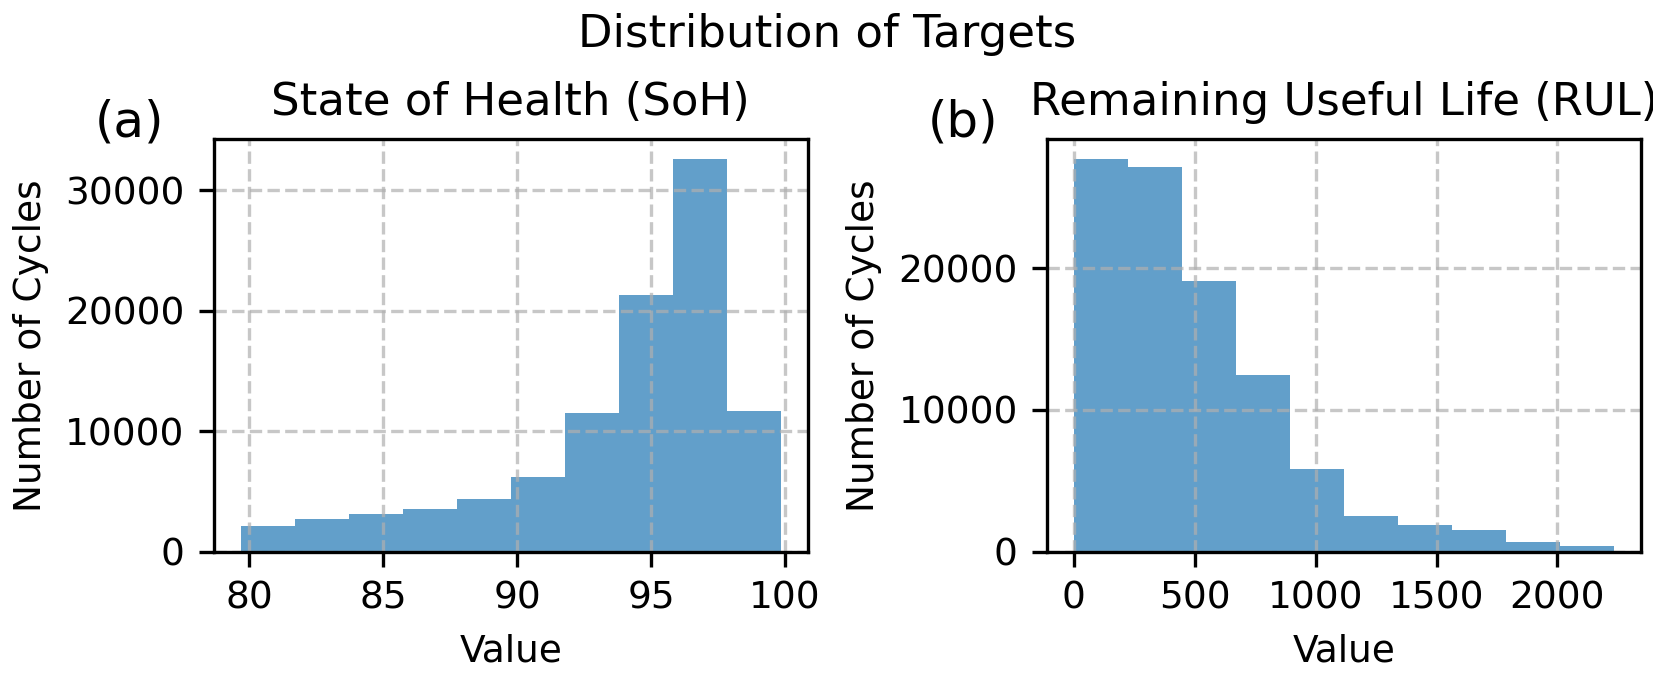
\includegraphics[width=0.8\textwidth]{_img_targets_distribution.png}
    \caption{Distributions of the target variables: (a) \acf{soh} and (b) \acf{rul}, showing the number of cycles across different values.}
    \label{fig:targets_distribution}
\end{figure}

\section{Data Analysis} \label{sec:data_analysis}
Building upon the dataset description provided in the previous section, this section presents an exploratory data analysis of the cycling data from 124 commercial \acf{lfp} batteries, as detailed in reference \cite{sev2019}. The analysis focuses on characterizing the voltage, current, temperature, and capacity measurements under the fast-charging protocols described earlier, with an emphasis on their evolution over the cells' lifecycle. These insights are critical for understanding battery degradation patterns and informing the development of machine learning models for estimating \acf{soh} and \acf{rul}. The dataset, organized into three batches with varying fast-charging protocols, provides a comprehensive basis for analyzing the impact of high C-rates and full \acf{dod} protocols, despite the limitations noted, such as controlled laboratory conditions and inconsistent temperature measurements.

The behavior of voltage, current, and temperature during a representative charge-discharge cycle is illustrated in Figure \ref{fig:voltage_current_temperature}, using the first cycle of the 32nd cell from Batch 2 as an example. This cell follows a 5.2C(50\%)-4.25C protocol, where charging involves a constant current (CC) of 5.2C until 50\% \acf{soc}, followed by 4.25C until 80\% \ac{soc}, as described in the dataset's experimental setup. After a 5-minute rest period, a 1C CC step continues until it reaches the upper voltage cutoff of 3.6 V, transitioning to constant voltage (CV) charging with naturally decreasing current until 100\% \ac{soc}. Discharge occurs at a constant 4C current until the lower voltage cutoff of 2.0 V is reached, this is followed by CV discharge until current reaches a cutoff of C/50 (in the case of Batch 2), which represents  full discharge. 

%Figure \ref{fig:temperature_and_capacities} showcases temperature along side charge and discharge capacity over the course of a given cycle. Though temperature peaks coincide with periods of charging and discharging, with the rate of temperature increase correlating with current intensity. During the rest period, the temperature drops, and during the 1C CC charging phase, it stabilizes, likely due to balanced heat generation and dissipation in the 30 °C chamber. This pattern is consistent with the discharge phase, where temperature rises with applied current and stabilizes during CV discharge. Although the observed correlation between temperature and the integral of current (i.e., capacity exchange) highlights that temperature can serve as a useful indicator of \ac{soc}, it should be noted that this relation partly reflects the specific experimental conditions -— namely constant charge/discharge profiles under controlled ambient temperature—and may not generalize to all operating scenarios.


\begin{figure}[H]
    \centering
    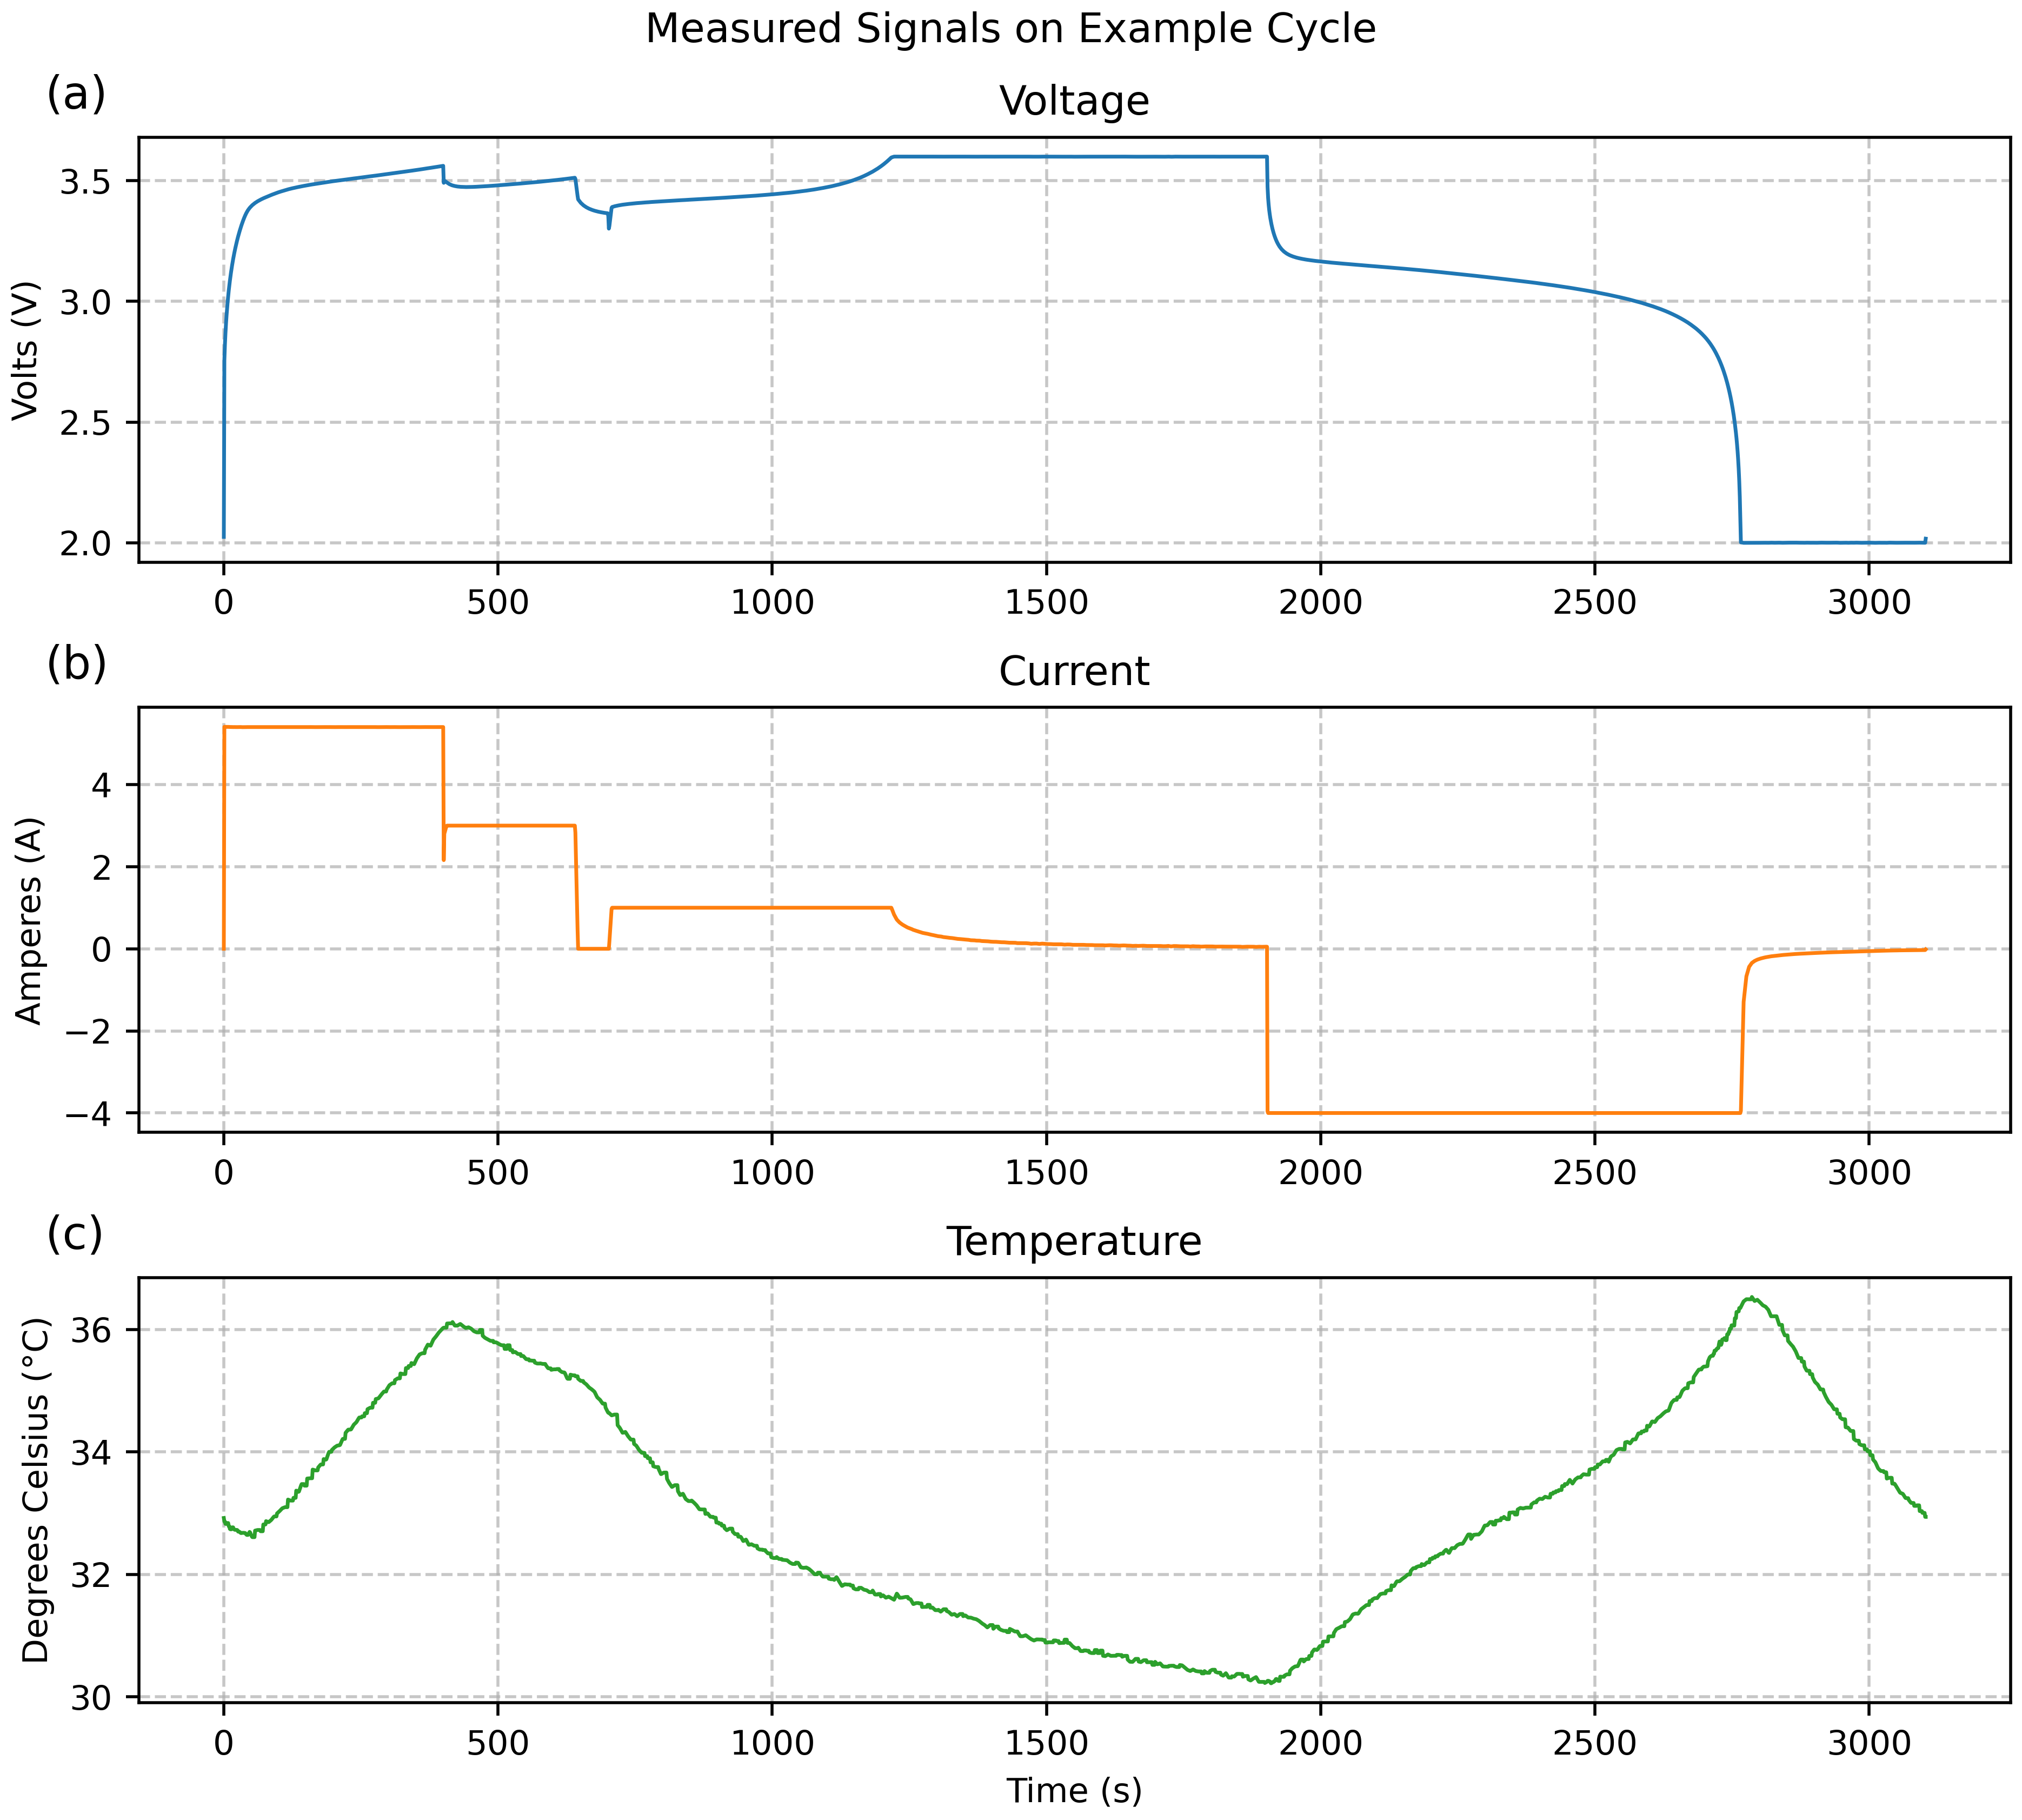
\includegraphics[width=1\textwidth]{_img_voltage_current_temperature.png}
    \caption{Voltage, current, and temperature profiles for a single cycle of the 32nd cell from Batch 2, following a 5.2C(50\%)-4.25C protocol. (a) Voltage, (b) Current, (c) Temperature.}
    \label{fig:voltage_current_temperature}
\end{figure}


\iffalse
\begin{figure}[H]
    \centering
    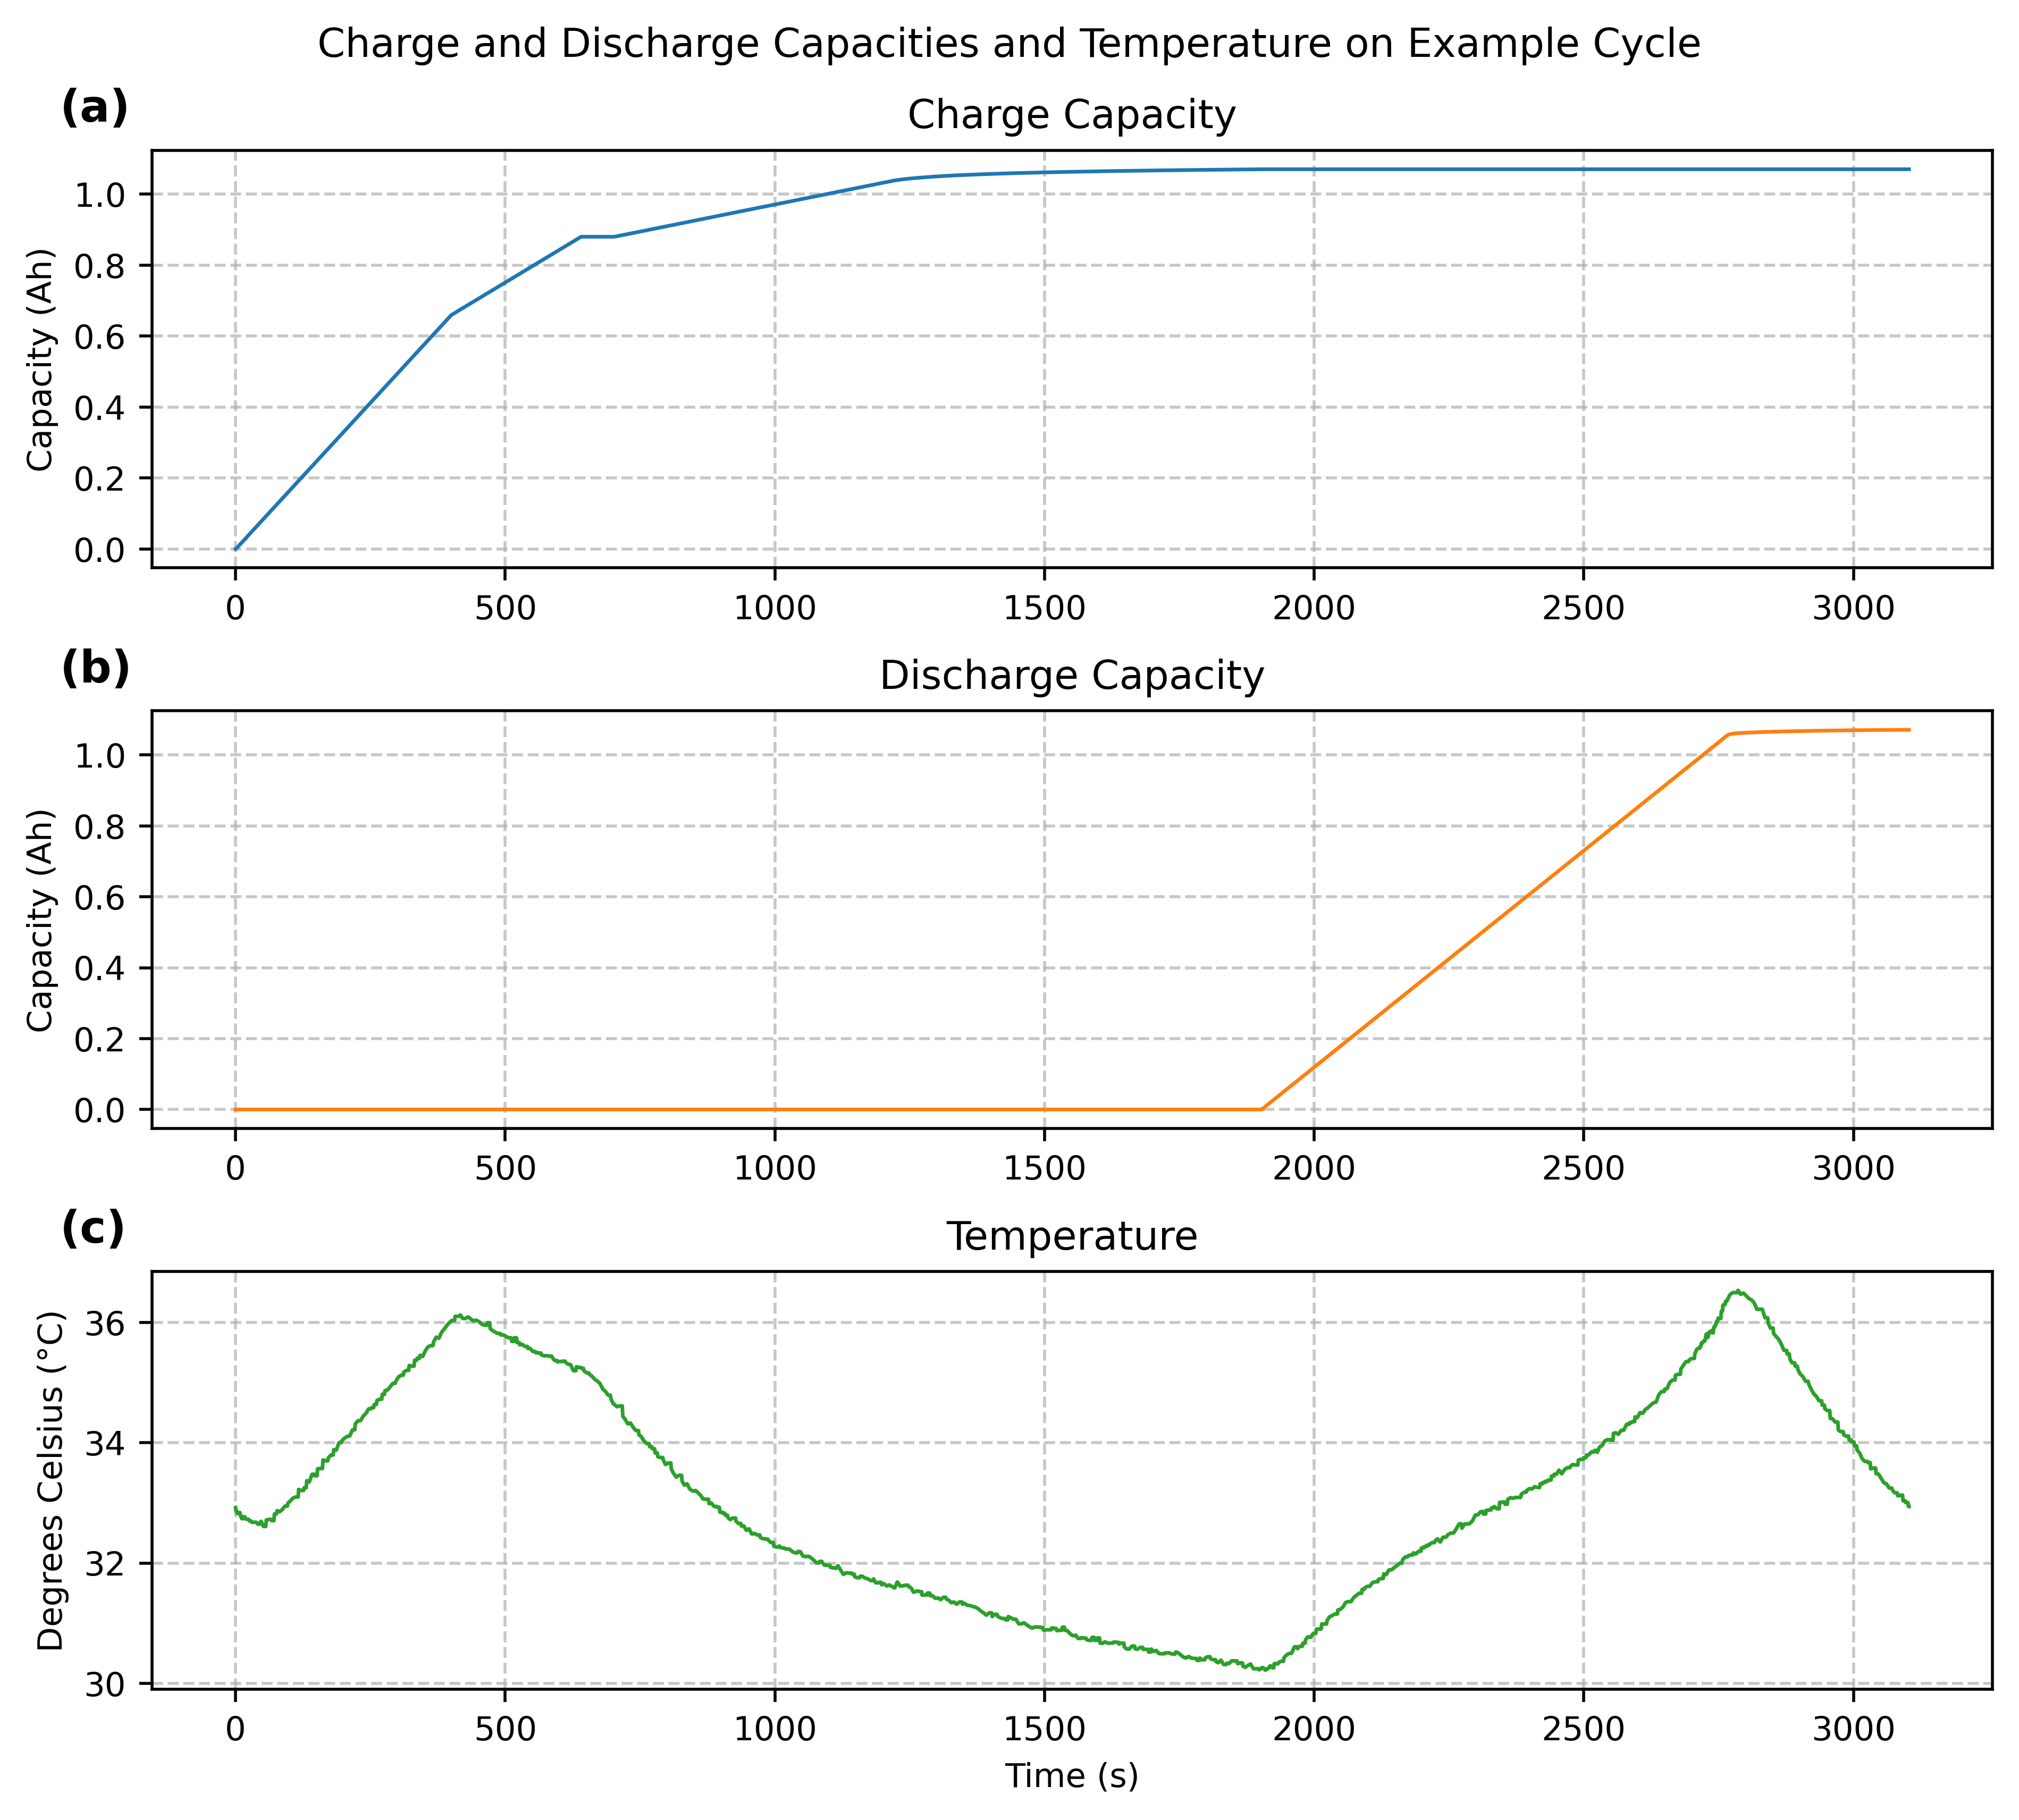
\includegraphics[width=1\textwidth]{_img_temperature_and_capacities.png}
    \caption{Correlation between capacity and temperature. (a) Charge capacity, (b) Discharge capacity, (c) Temperature. \todo[size=\tiny]{[R2] Figure shows relationship between Temperature and Capacity, This is not discussed in the text, however.}}
    \label{fig:temperature_and_capacities}
\end{figure}
\fi


The evolution of \ac{soh} across the cells' lifecycle, as defined in the dataset description, is depicted in Figure \ref{fig:all_cell_soh}. Most cells start with an \ac{soh} near 100\% and exhibit a gradual decline until a characteristic "knee point", after which the degradation rate accelerates. This behavior is consistent across all batches, despite variations in rest periods and cutoff currents. The cycle life distribution, shown in Figure \ref{fig:cycle_life_distribution}, indicates that most cells (mode) reach \acf{eol} at around 500 cycles, while the average cycle life is aroung 700 cycles. This is significantly shorter than the cycle lifes described elsewhere in the literature, this is likely due to the aggressive 4C discharge and full DoD protocols described earlier. As noted in the dataset limitations, this accelerated aging may not reflect real-world conditions. An anomaly around cycle 250 in Batch 2, caused by an 8-hour rest period due to a computer restart, manifests as capacity spikes, introducing outliers in voltage, current, and temperature measurements. These outliers are removed during data preprocessing to ensure robust model training.

\begin{figure}[H]
    \centering
    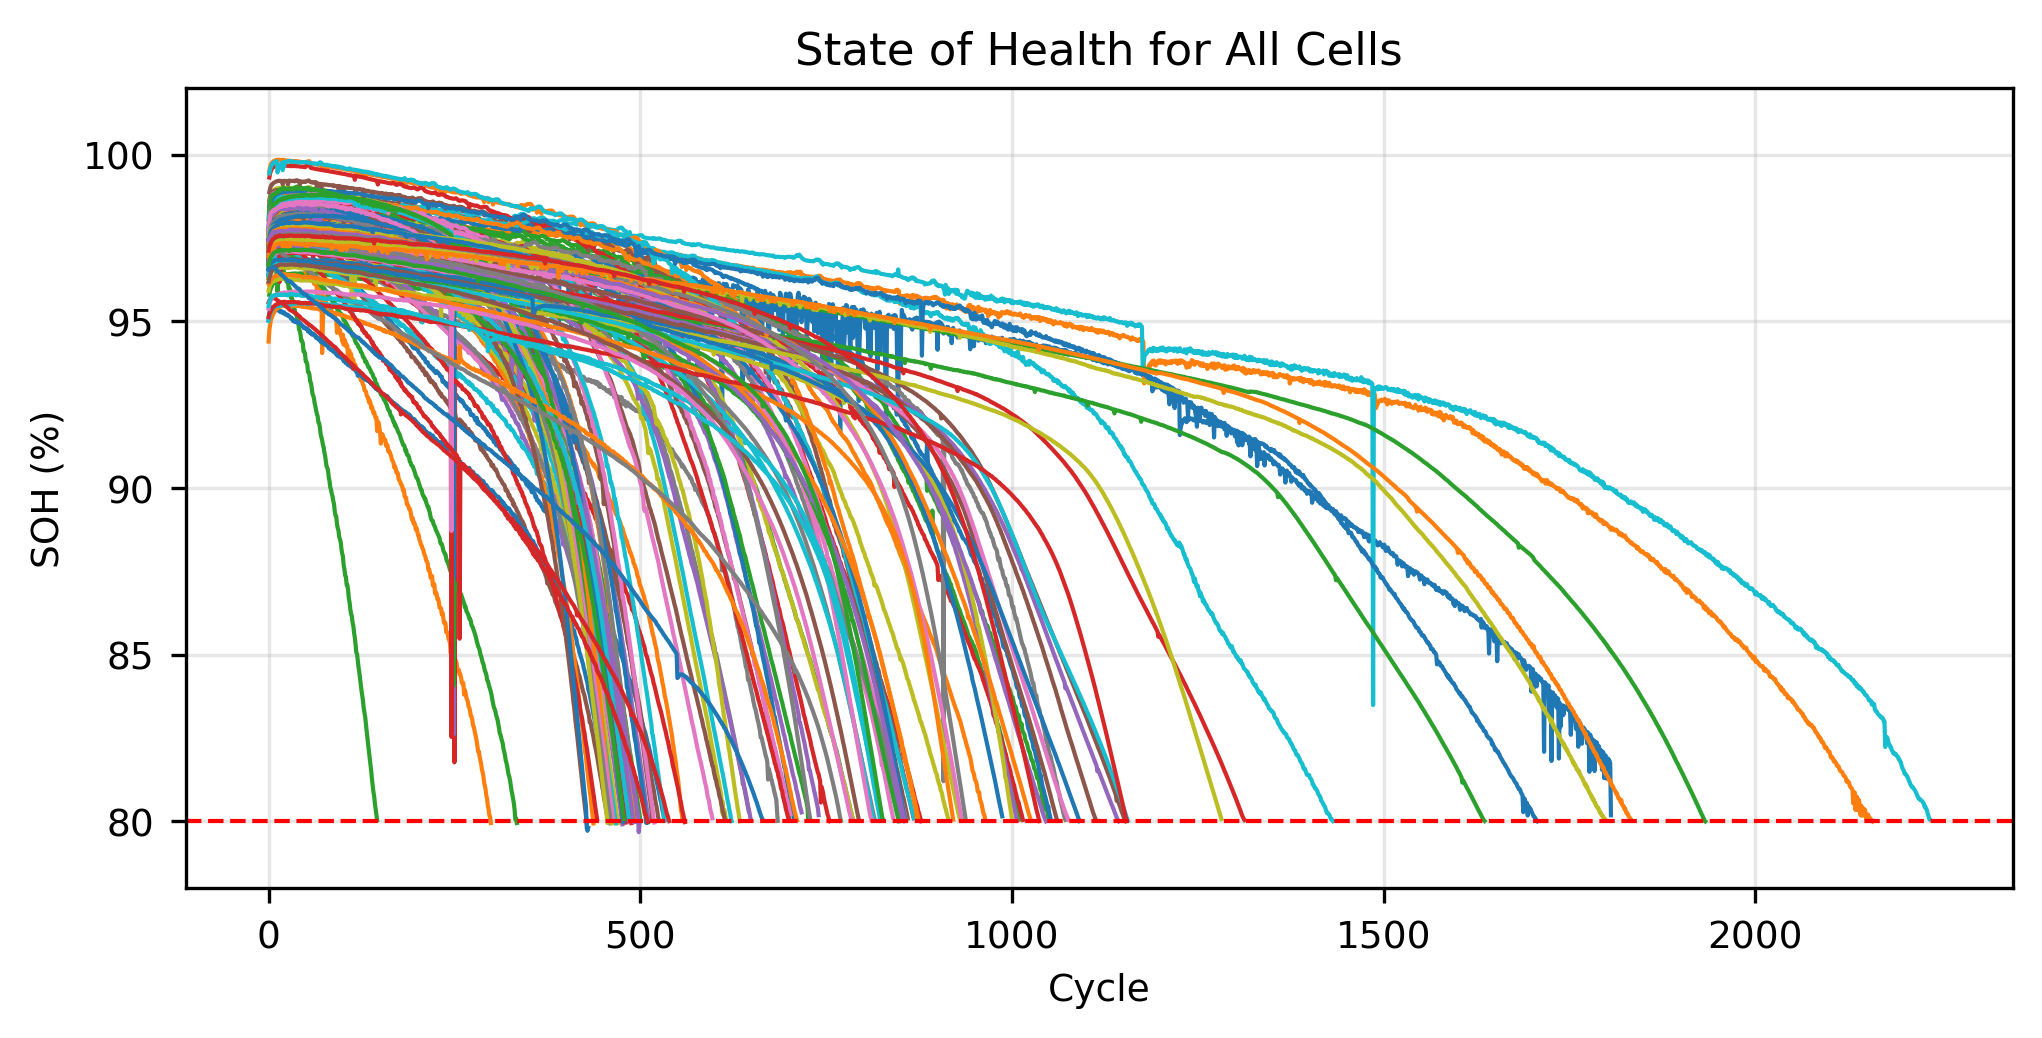
\includegraphics[width=0.8\textwidth]{_img_all_cell_soh.png}
    \caption{State of Health (SOH) evolution for all cells across Batches 1, 2, and 3.}
    \label{fig:all_cell_soh}
\end{figure}

\begin{figure}[H]
    \centering
    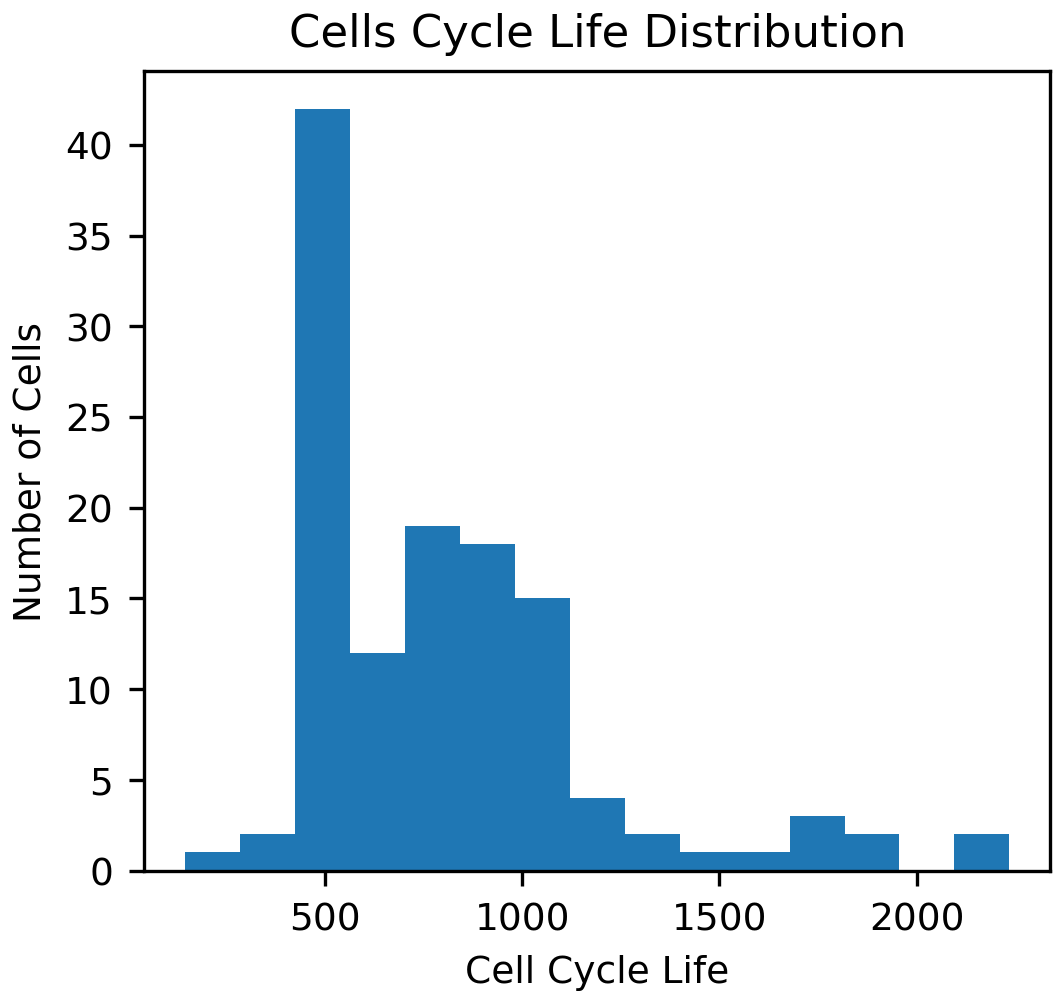
\includegraphics[width=0.8\textwidth]{_img_cycle_life_distribution.png}
    \caption{Histogram of cycle life distribution across all cells.}
    \label{fig:cycle_life_distribution}
\end{figure}


The impact of aging on voltage and current profiles is examined in Figure \ref{fig:voltage_current_begin_and_end}, which compares these signals at the beginning, middle, and end the life of the 32nd cell from Batch 2 as an example. At the start (Figure \ref{fig:voltage_current_begin_and_end}(a)), the profiles align with the defined fast-charge protocol. By mid-life (Figure \ref{fig:voltage_current_begin_and_end}(b)), changes are subtle, but at EoL (Figure \ref{fig:voltage_current_begin_and_end}(c)), increased internal resistance, measured as described in the dataset, causes the 3.6 V and 2.2 V thresholds to be reached earlier, leading to extended CV phases with reduced current. This results in shorter cycle durations at EoL, reflecting the reduced capacity observed post-knee point in Figure \ref{fig:all_cell_soh}.

\begin{figure}[H]
    \centering
    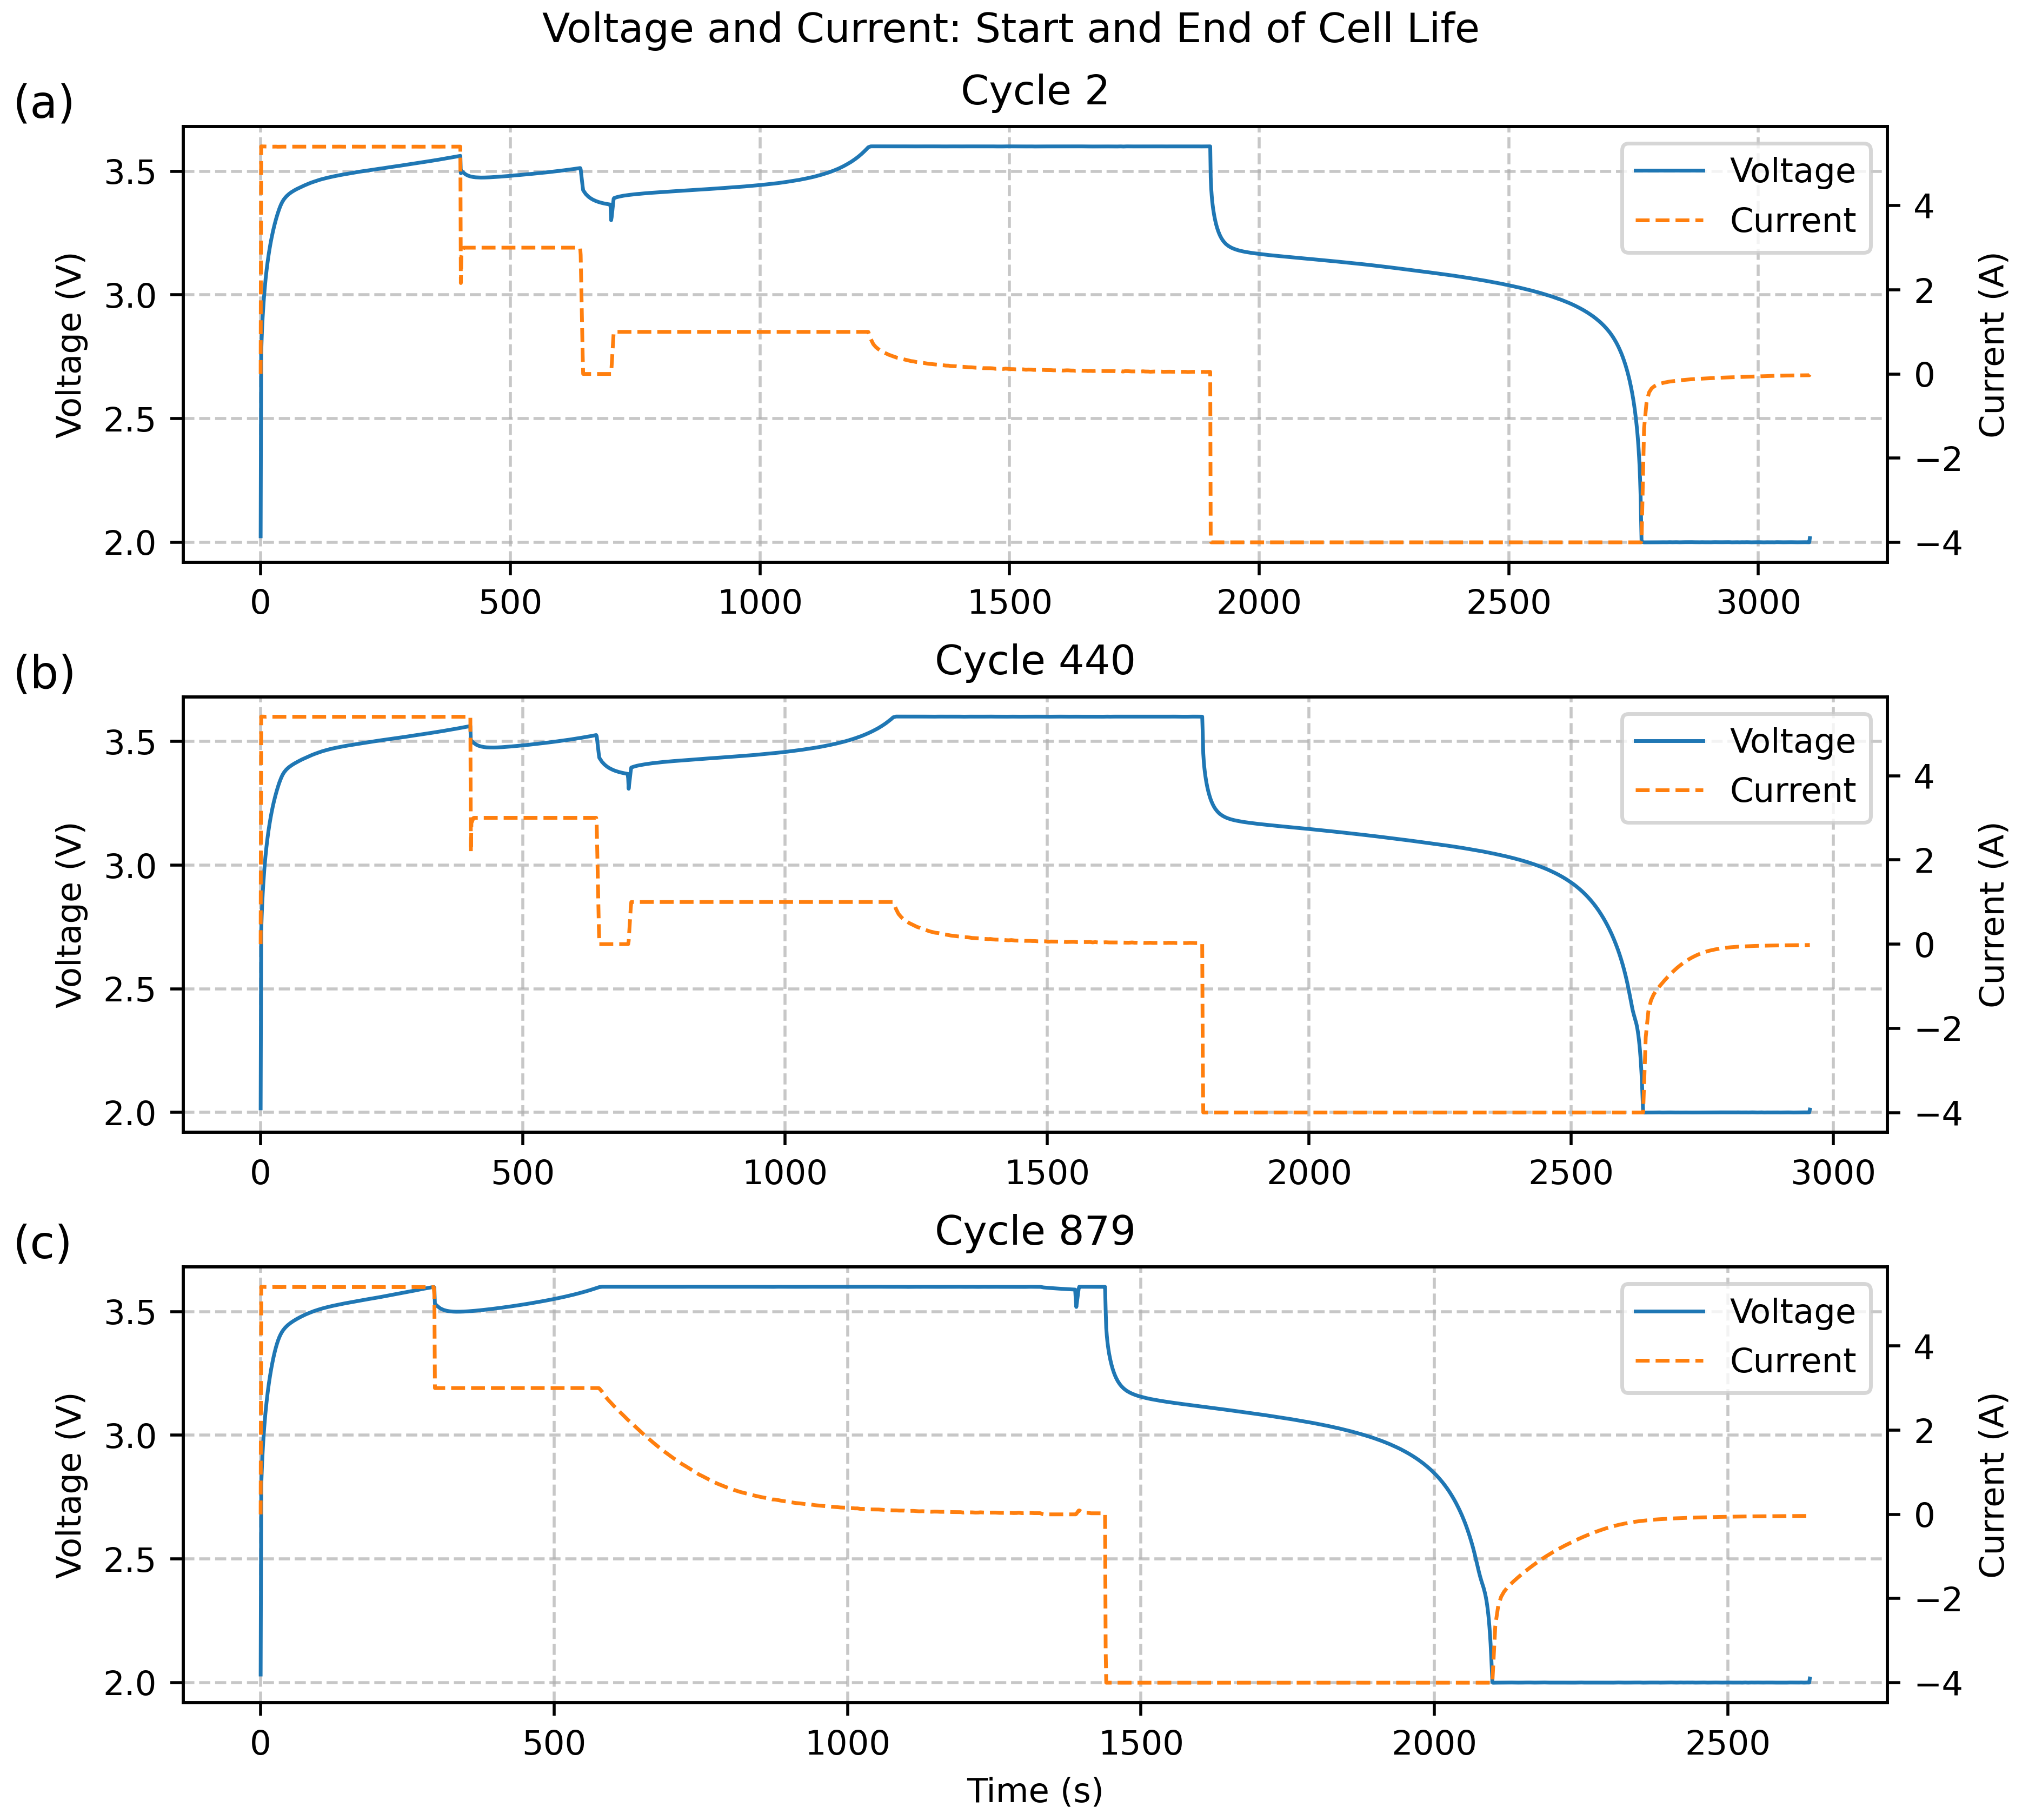
\includegraphics[width=1\textwidth]{_img_voltage_current_begin_and_end.png}
    \caption{Voltage and current profiles at different stages of cell life. (a) Beginning, (b) Middle, (c) End.}
    \label{fig:voltage_current_begin_and_end}
\end{figure}


A detailed visualization of the fast-charge protocol is provided in Figure \ref{fig:charge_steps}, with color-coded regions highlighting the CC1, CC2, CC3, CV charge, discharge, and rest periods, as described in the experimental setup. For Batch 2, the protocol includes a 5-minute rest after 80\% \ac{soc} and post-discharge, with C/50 cutoff currents for CV phases. This structured protocol ensures consistency across cycles, facilitating the analysis of aging effects.

\begin{figure}[H]
    \centering
    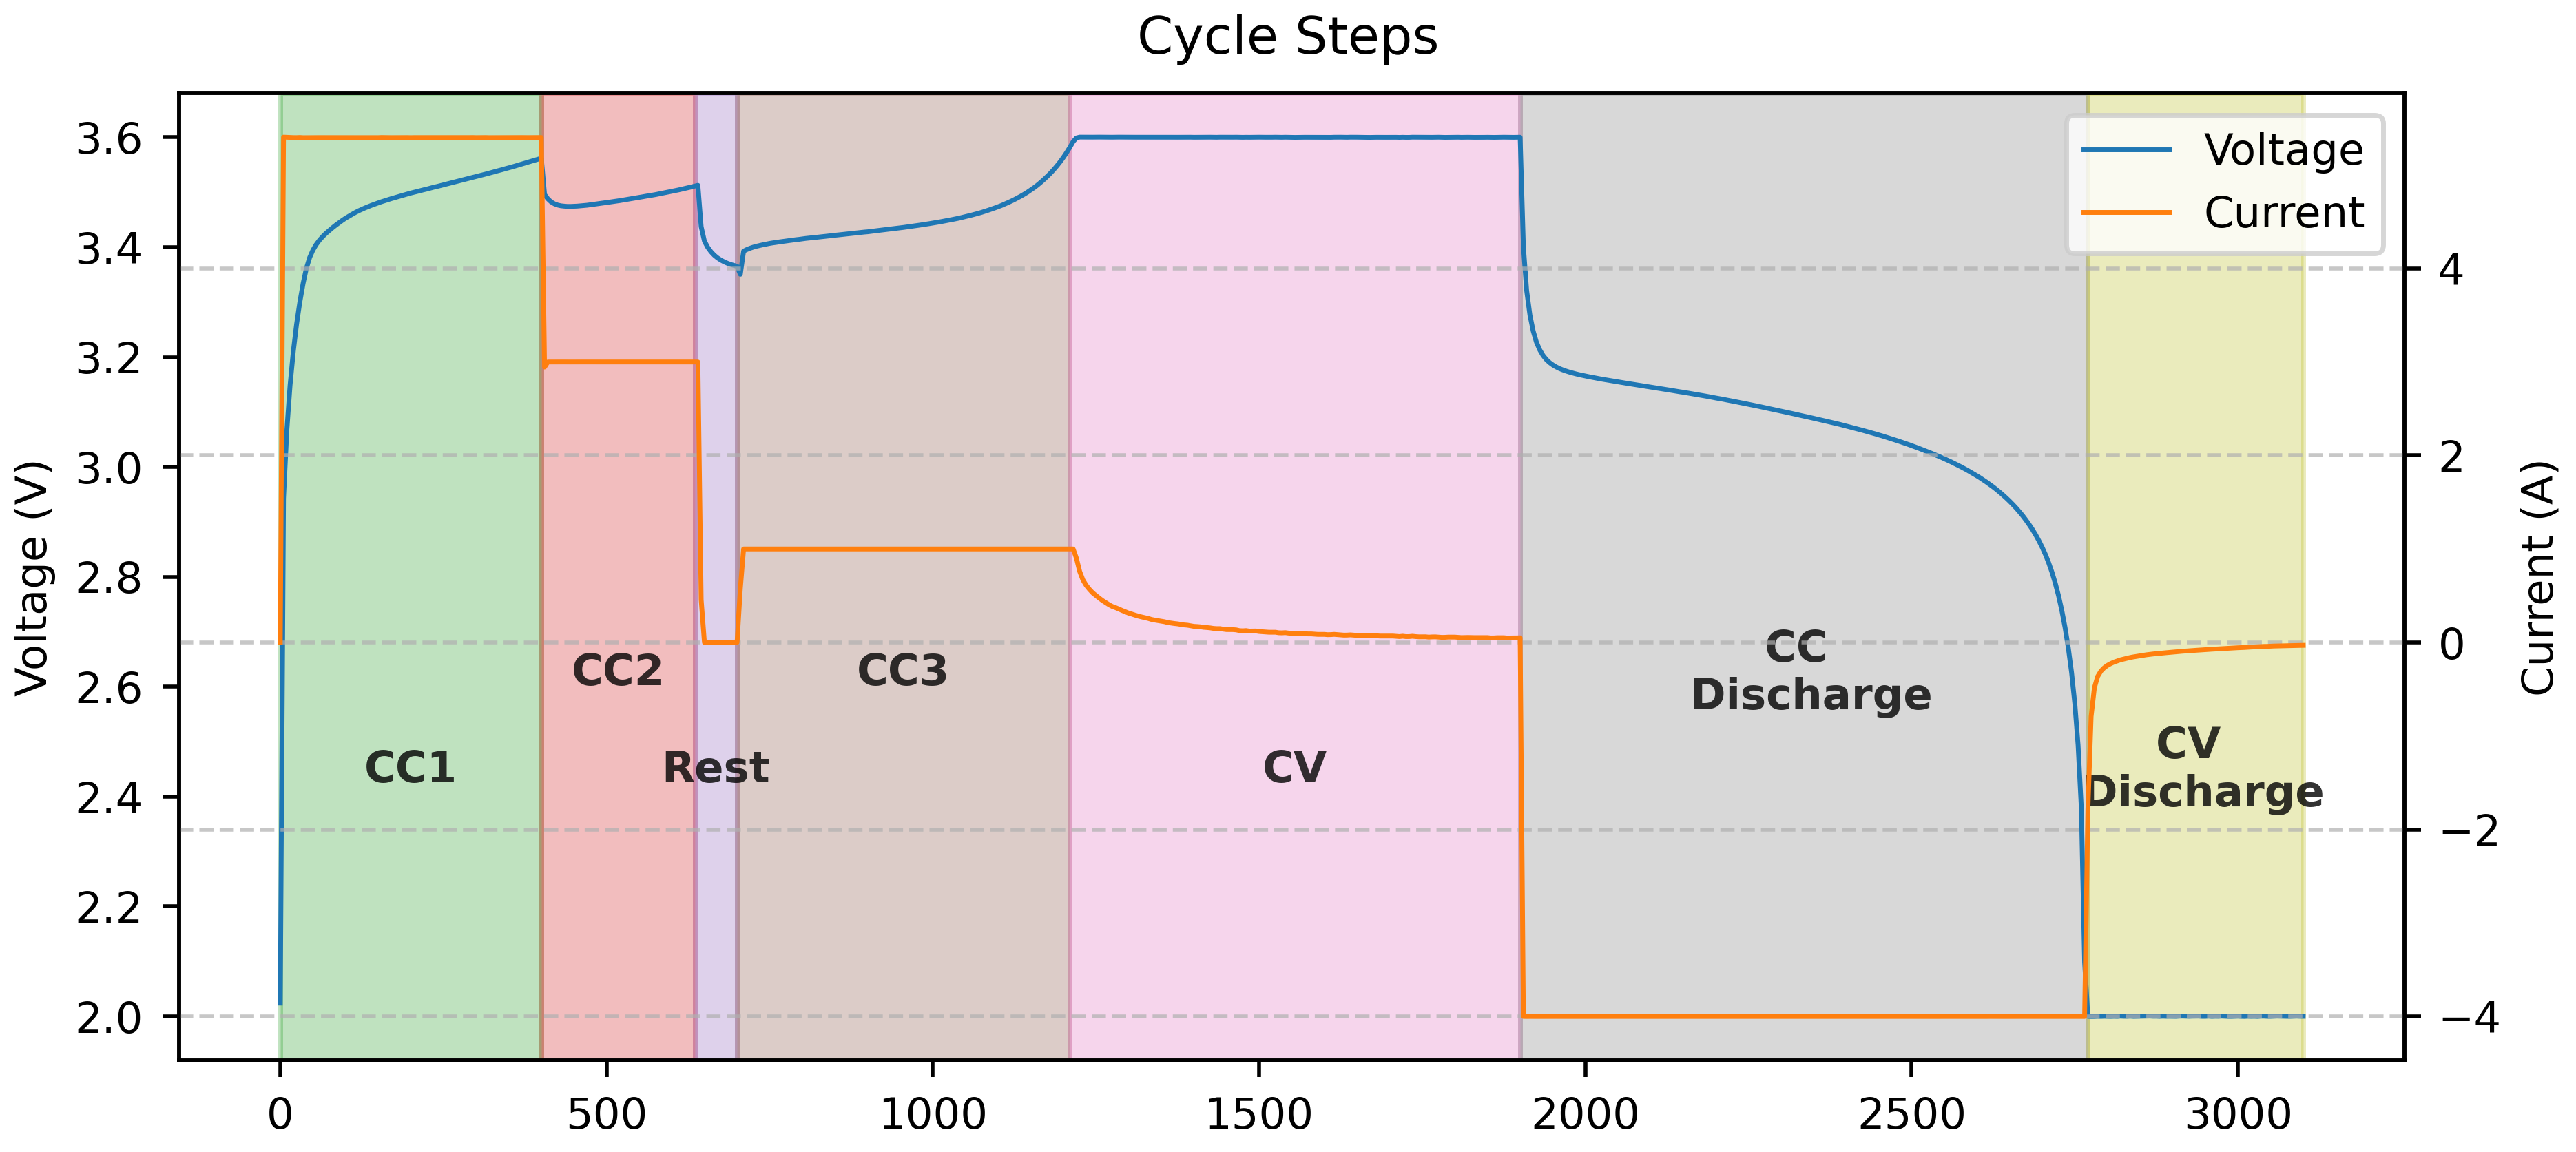
\includegraphics[width=1\textwidth]{_img_charge_steps.png}
    \caption{Fast-charge protocol with color-coded phases: CC1, CC2, CC3, CV charge, discharge, and rest periods.}
    \label{fig:charge_steps}
\end{figure}


The evolution of voltage, current, and temperature across multiple cycles is shown in Figure \ref{fig:signals_through_cycles}, using a Batch 2 cell as an example. The most significant changes occur near EoL (cycle 501), where increased internal resistance, as measured at 80\% \ac{soc}, leads to earlier CV phases and higher peak temperatures during discharge, likely due to enhanced Joule heating. This aligns with the dataset’s observation of thermocouple variability, which may amplify temperature measurement noise at \ac{eol}.

\begin{figure}[H]
    \centering
    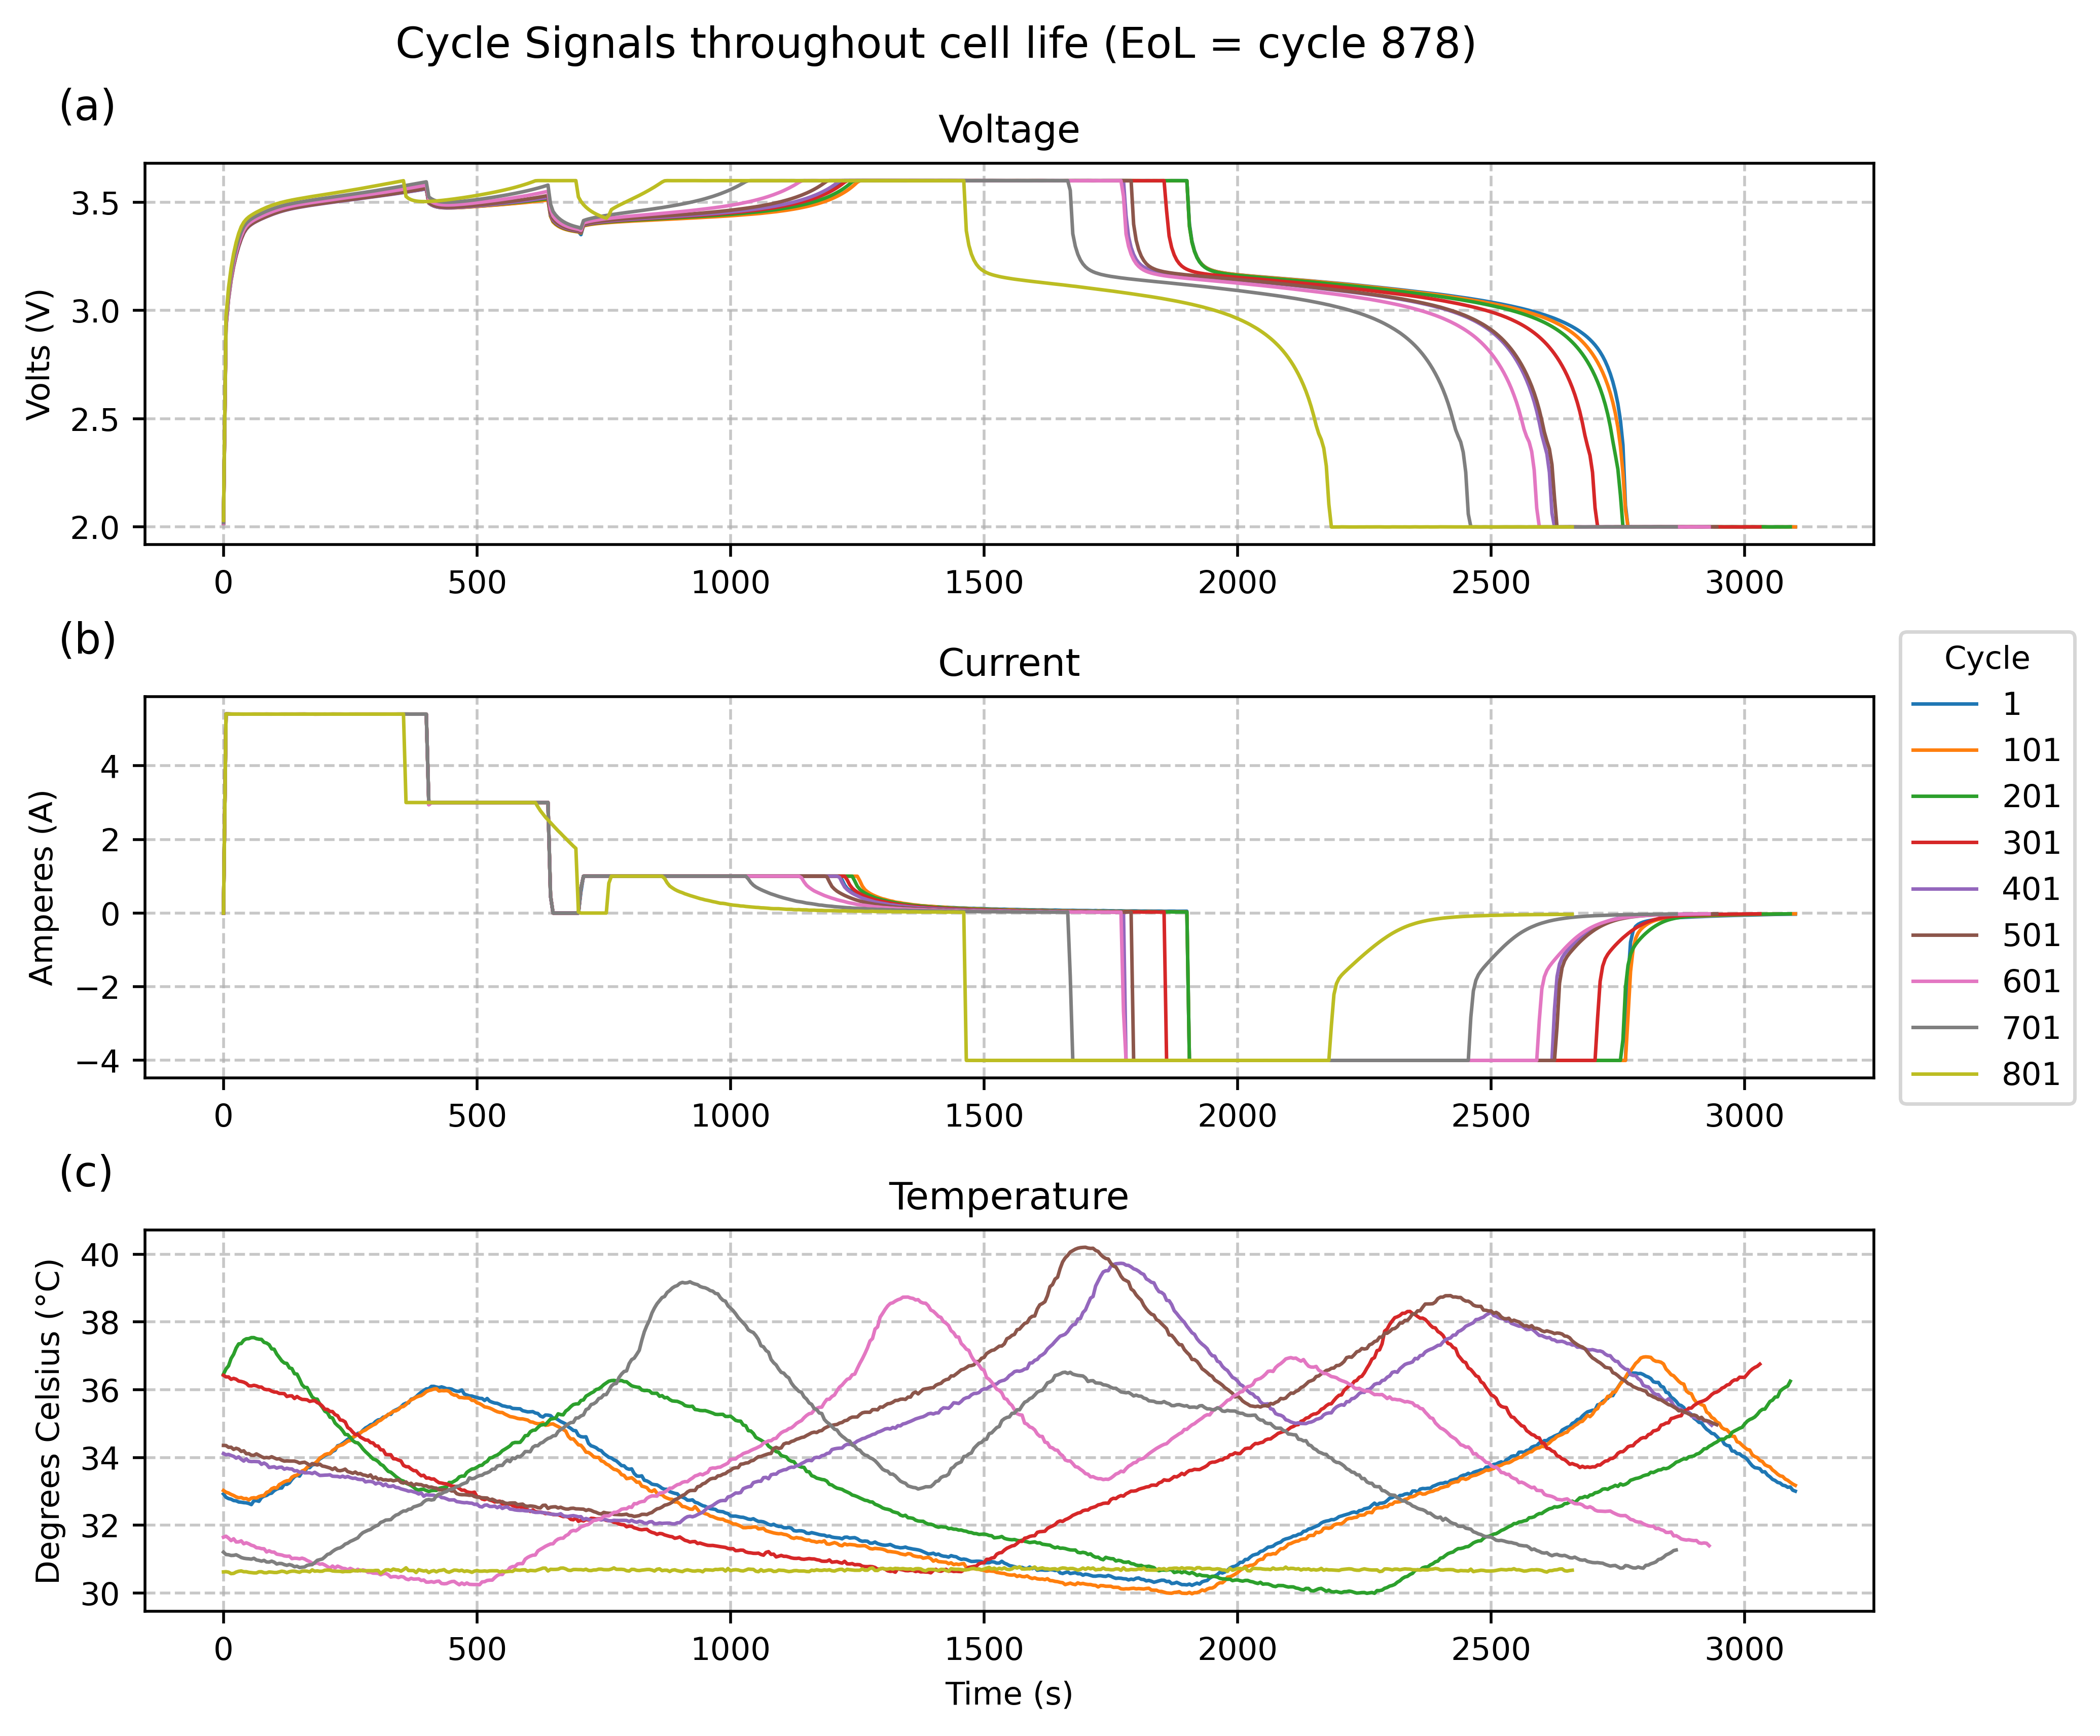
\includegraphics[width=1\textwidth]{_img_signals_through_cycles.png}
    \caption{Voltage, current, and temperature profiles across multiple cycles, highlighting aging effects.}
    \label{fig:signals_through_cycles}
\end{figure}


To assess the impact of fast-charge protocols on cycle life, a correlation analysis was performed across the dataset's range of one-step and two-step policies. Figure \ref{fig:charge_current_and_cycle_life} shows a scatter plot of the mean charge C-rate versus cycle life. The mean C-rate, $\overline{C}$, is defined as the weighted average of the constant-current (CC) steps up to 80\% \ac{soc}:

\begin{equation}
\overline{C} = \frac{\sum_{i} C_i \, \Delta \mathrm{SOC}_i}{0.8},
\end{equation}

where $C_i$ is the C-rate of the $i$-th step and $\Delta \mathrm{SOC}_i$ is the fraction of state of charge (SOC) covered by that step. For example, a 4C(50\%)-5C protocol yields $\overline{C} = (4 \times 0.5 + 5 \times 0.3)/0.8$. A Pearson correlation coefficient of $R = -0.61$ indicates a moderate negative correlation, confirming that higher charge currents, as applied across all batches, accelerate aging, consistent with the dataset's high C-rate conditions.


\begin{figure}[H]
    \centering
    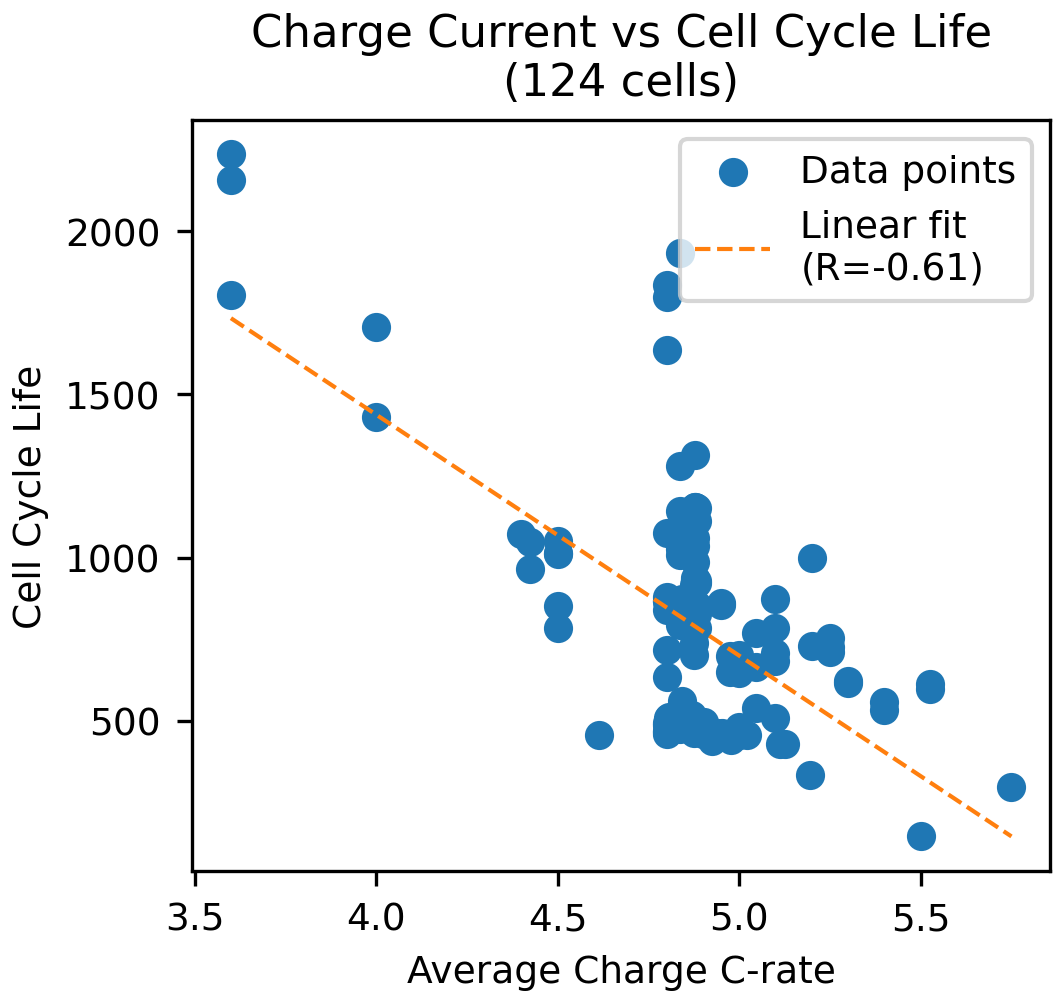
\includegraphics[width=0.5\textwidth]{_img_charge_current_and_cycle_life.png}
    \caption{Scatter plot of average charge C-rate versus cycle life, with Pearson correlation coefficient $R = -0.61$.}
    \label{fig:charge_current_and_cycle_life}
\end{figure}


Further analysis in Figure \ref{fig:charge_steps_area_diff} evaluates the difference in charge "area" between the second and first constant-current (CC) steps. The goal of this analysis is to assess how different current intensities applied at different \acp{soc} influence battery life. The area difference, $\Delta A$, is defined as

\begin{equation}
\Delta A = C_2 \, \Delta \mathrm{SOC}_2 - C_1 \, \Delta \mathrm{SOC}_1,
\end{equation}

where $C_1$ and $C_2$ are the C-rates of the first and second steps, respectively, and $\Delta \mathrm{SOC}_1$ and $\Delta \mathrm{SOC}_2$ are the corresponding fractions of state of charge (SOC) covered. For example, a 4C(50\%)-3C protocol yields $\Delta A = 3 \times 0.3 - 4 \times 0.5$. A Pearson correlation coefficient of $R = 0.38$ indicates a weak positive correlation, suggesting that the order and duration of fast-charge steps have minimal impact on cycle life compared to the overall charge current magnitude.

\begin{figure}[H]
    \centering
    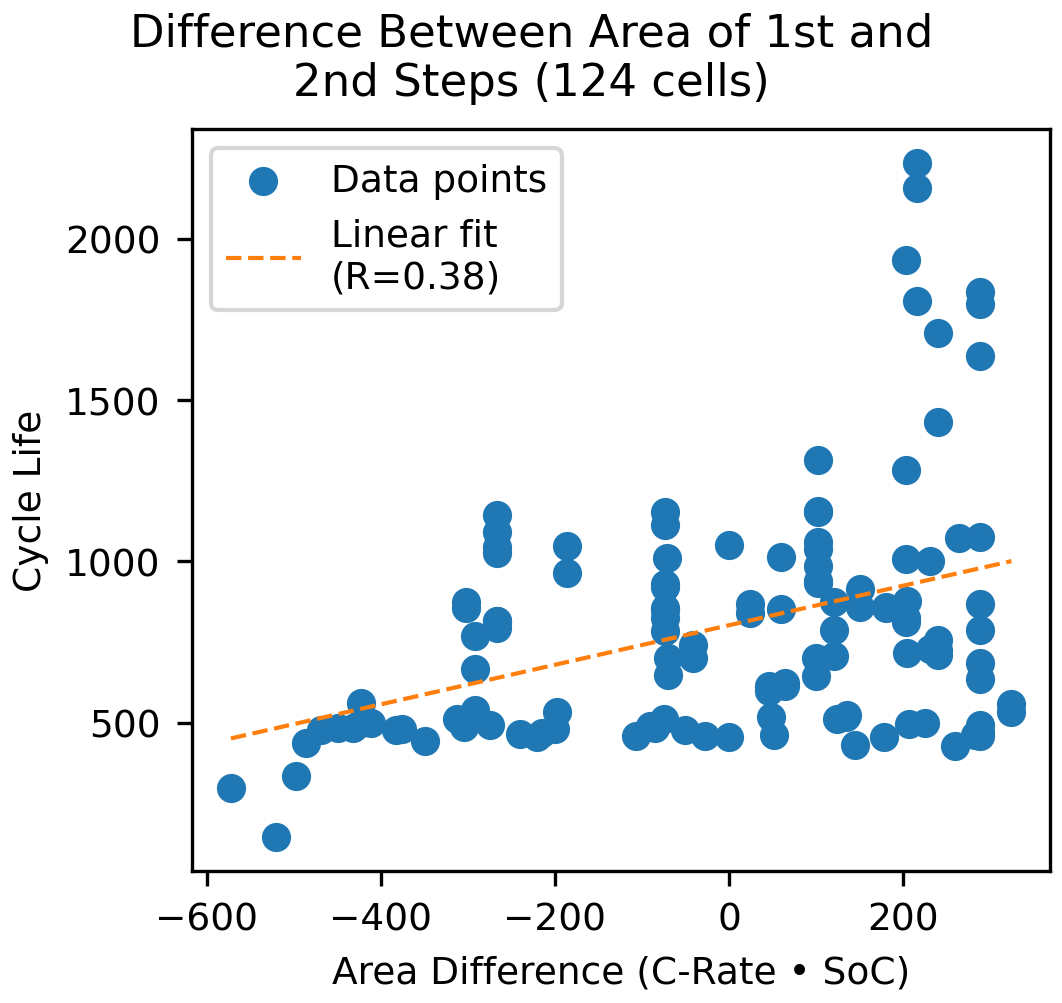
\includegraphics[width=0.5\textwidth]{_img_charge_steps_area_diff.png}
    \caption{Scatter plot of charge step area difference versus cycle life, with Pearson correlation coefficient $R = 0.38$.}
    \label{fig:charge_steps_area_diff}
\end{figure}


In summary, the exploratory data analysis, grounded in the dataset’s detailed measurements and experimental conditions, reveals key trends in \ac{lfp} battery behavior under fast-charging protocols. Temperature strongly correlates with capacity exchange, supporting its use as an \ac{soc} indicator, though measurement reliability is limited by thermocouple inconsistencies. \ac{soh} degradation accelerates post-knee point, with cycle life averaging 700 cycles due to aggressive testing conditions, as noted in the dataset limitations. Aging significantly alters voltage and current profiles, with increased internal resistance driving earlier CV phases and shorter cycles at \ac{eol}. Correlation analyses confirm that higher charge currents reduce cycle life, while step order has minimal impact. These findings, despite the dataset’s constraints (e.g., single chemistry, controlled environment), provide a robust foundation for developing machine learning models to predict \ac{rul} and \ac{soh}, leveraging the observed relationships between measurable signals and degradation patterns.

\input{__sec05_feature_extraction}
\input{__sec06_models}
\section{Model Training and Optimization}
\label{sec:optimiation}
% Introducing the purpose and approach
This section describes the methodology for training and optimizing machine learning models to estimate the \acf{soh} and \acf{rul} of lithium-ion batteries, utilizing the features extracted from the dataset detailed in prior sections. Machine learning models are mathematical frameworks that identify patterns in data to predict outcomes, here mapping cycle features to \ac{soh} or \ac{rul}. Separate models were trained for \ac{soh} and \ac{rul} to avoid the complexity of joint estimation, focusing on generalization to cells not included in the training data, a critical requirement for applications such as battery management systems in electric vehicles or energy storage.

\subsection{Data Preparation}

% Describing train-test split
To ensure models generalize to unseen cells, the dataset of 124 cells was partitioned into training and test sets by randomly assigning entire cells, preventing any cell’s data from appearing in both sets. This approach mitigates data leakage, where models could exploit specific cell behaviors, leading to overly optimistic performance estimates. As presented in Table \ref{tab:splits_cells_summary}, the training set comprises 99 cells (80,618 cycles), and the test set includes 25 cells (18,480 cycles), adhering to an approximate 80:20 split, a standard practice to balance training data availability with robust evaluation.

\begin{table}[h]
    \centering
    \caption{Division of cells and total samples (cycles) into training and test sets.}
    \label{tab:splits_cells_summary}
    \begin{tabular}{lrr}
        \toprule
        \textbf{Partition} & \textbf{No. of Cells} & \textbf{Total Samples (Cycles)} \\
        \midrule
        Training & 99 & 80618 \\
        Test     & 25 & 18480 \\
        \midrule
        \textbf{Total} & \textbf{124} & \textbf{99098} \\
        \bottomrule
    \end{tabular}
\end{table}

% Describing feature scaling
Features were standardized using Standard Scaling, transforming each feature to have a mean of zero and a \acf{std} of one, based on statistics derived from the training set. Standardization ensures that features with different scales (e.g., voltage mean in volts vs. unitless kurtosis) contribute equally to model training, preventing bias toward larger-magnitude features. The scaling parameters from the training set were applied to the test set to maintain consistency, mirroring real-world scenarios where new data are processed using established parameters.

\subsection{Model Training and Evaluation}

% Describing model training
Model training entails optimizing internal parameters (weights) to minimize prediction errors on the training data. In this study, models learn to map cycle features (e.g., voltage mean, temperature \ac{std}) to \ac{soh} or \ac{rul}, minimizing the \acf{mse}, which quantifies the average squared difference between predicted and actual values, penalizing larger errors more heavily. Ground truth \ac{soh} and \ac{rul} values from all cycles of the 99 training cells were utilized, leveraging the dataset’s full-life data. In practical applications, full-life data may be unavailable, necessitating alternative approaches: (1) personalized models trained on early cycles of a specific cell for its future predictions, or (2) general models trained on early cycles from multiple cells, applicable to any cell at any stage. These methods are challenging, as early-cycle data may not capture aging patterns, a significant hurdle in battery research. Given the availability of full-life data, this study uses all cycles from training cells to assess feature and model performance for unseen cells, aligning with the objective of generalization.

% Describing model evaluation
Model performance was evaluated by generating predictions for the test set (25 unseen cells) and comparing them to ground truth \ac{soh} and \ac{rul} values using three metrics:

\begin{itemize}
    \item \textbf{\acf{mae}:} The average absolute difference between predicted and actual values, expressed in the target’s units (e.g., percentage for \ac{soh}, cycles for \ac{rul}).
    \begin{equation}
        \mathrm{MAE} = \frac{1}{n} \sum_{i=1}^{n} \left| y_i - \hat{y}_i \right|
        \label{eq:mae}    
    \end{equation}
    
    \item \textbf{\acf{rmse}:} The square root of \ac{mse}, emphasizing larger errors while maintaining the target’s units.
    \begin{equation}
        \mathrm{RMSE} = \sqrt{\frac{1}{n} \sum_{i=1}^{n} (y_i - \hat{y}_i)^2}
        \label{eq:rmse}
    \end{equation}
    
    \item \textbf{\acf{r2}:} A metric from 0 to 1, indicating the proportion of variance in the target explained by the model, with 1 representing perfect predictions.
    \begin{equation}
        R^2 = 1 - \frac{\sum_{i=1}^{n} (y_i - \hat{y}_i)^2}{\sum_{i=1}^{n} (y_i - \bar{y})^2}
        \label{eq:r2}
    \end{equation}
\end{itemize}

For inference, models require voltage, current, and temperature signals from a single full charge-discharge cycle, sampled at 1 Hz or higher, processed into the 15 features described previously.

\subsection{Hyperparameter Optimization}

% Defining hyperparameters and optimization approach
Machine learning models rely on hyperparameters—configurable settings that define their structure or learning process, such as the number of trees in a Random Forest or the learning rate in a neural network. Unlike model weights, hyperparameters are set prior to training and typically determined empirically. To automate this process, the Tree-structured Parzen Estimator (TPE) \cite{tpe_2011}, a Bayesian optimization algorithm, was employed. TPE iteratively samples from a predefined hyperparameter space, balancing exploration of new configurations with exploitation of previously successful ones.

To balance predictive accuracy and model generalization, a custom cost function was adopted, combining validation error and the generalization gap. The objective to minimize is defined as:

\begin{equation}
    \mathcal{L} = \mathrm{RMSE}_{\text{val}} + \frac{\left| \mathrm{RMSE}_{\text{train}} - \mathrm{RMSE}_{\text{val}} \right|}{\mathrm{RMSE}_{\text{val}}}
\end{equation}

where the first term, \(\text{RMSE}_{\text{val}}\), is the root mean square error on the validation folds, as defined by Equation \ref{eq:rmse}, and the second term, %\(\frac{|\text{RMSE}_{\text{train}} - \text{RMSE}_{\text{val}}|}{\text{RMSE}_{\text{val}}}\), 
represents the relative generalization gap between training and validation errors. This formulation penalizes both high validation errors and large discrepancies between training and validation performance, effectively discouraging overfitting while prioritizing predictive accuracy.

% Explaining cross-validation setup
Trials were evaluated using 5-fold Group K-Fold cross-validation. The 99 training cells were partitioned into 5 non-overlapping groups (based on cell ID), ensuring that all cycles from a given cell remained within the same fold to prevent data leakage. The final loss score is computed as the average of the defined loss across the 5 validation folds. Figure \ref{fig:kfold} illustrates the 5-fold cross-validation process adopted. In order speed up the cross validation process, a smaller training dataset, a subset of the full training dataset, is used during this step; the distribution of both SoH and RUL targets between both datasets is shown in Figure \ref{fig:subset_distributions}.

% Detailing early stopping strategy
To improve optimization efficiency and prevent unnecessary trials, an early stopping strategy was employed. If the cost does not improve for a fixed number of consecutive trials (patience = 10), the optimization process is halted. This ensures that exploration ceases when no meaningful improvement is observed.

\begin{figure}[H]
\centering
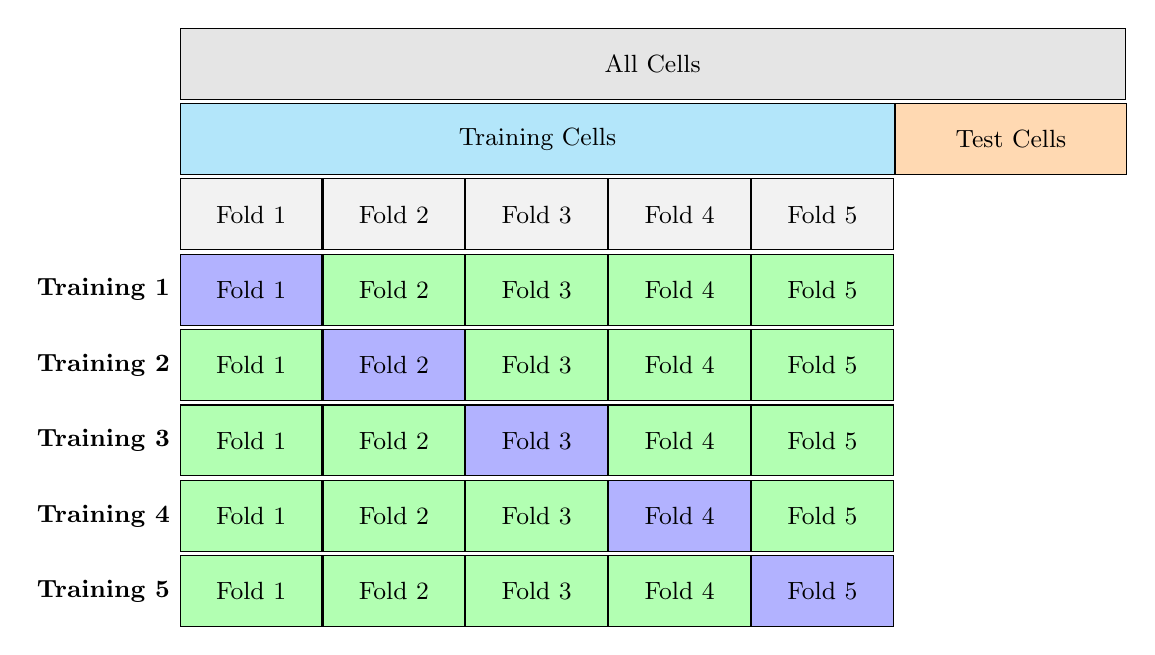
\begin{tikzpicture}[
    box/.style={rectangle, draw=black, minimum height=0.9cm, text centered, font=\small},
    fold/.style={rectangle, draw=black, minimum height=0.9cm, minimum width=1.8cm, text centered, font=\small},
    all_data/.style={box, fill=gray!20, minimum width=12cm},
    train_data/.style={box, fill=cyan!30, minimum width=9.075cm},
    test_data/.style={box, fill=orange!30, minimum width=2.925cm},
    foldtrain/.style={fold, fill=green!30},
    foldtest/.style={fold, fill=blue!30},
    legend/.style={font=\small\bfseries}
]
    % Top: Todos os dados
    \node[all_data] (all_data) {All Cells};
    % Segunda linha: divisão em treino e teste
    \node[train_data, below=0.5cm, at=(all_data.south west), anchor=west] (train_data) {Training Cells};
    \node[test_data, right=0cm, at=(train_data.east), anchor=west] (test_data) {Test Cells};
    % Terceira linha: cabeçalhos dos folds
    \node[fold, fill=gray!10, below=0.5cm, at=(train_data.south west), anchor=west] (foldh0) {Fold 1};
    \node[fold, fill=gray!10, right=0cm, at=(foldh0.east), anchor=west] (foldh1) {Fold 2};
    \node[fold, fill=gray!10, right=0cm, at=(foldh1.east), anchor=west] (foldh2) {Fold 3};
    \node[fold, fill=gray!10, right=0cm, at=(foldh2.east), anchor=west] (foldh3) {Fold 4};
    \node[fold, fill=gray!10, right=0cm, at=(foldh3.east), anchor=west] (foldh4) {Fold 5};
    
    % Validação cruzada com 5 linhas
    % Linha 1
    \node[legend, left=0.2cm, below=0.5cm, at=(foldh0.south west), anchor=east] (legend1) {Training 1};
    \node[foldtest, below=0.5cm, at=(foldh0.south west), anchor=west] (f11) {Fold 1};
    \node[foldtrain, right=0cm, at=(f11.east), anchor=west] (f12) {Fold 2};
    \node[foldtrain, right=0cm, at=(f12.east), anchor=west] (f13) {Fold 3};
    \node[foldtrain, right=0cm, at=(f13.east), anchor=west] (f14) {Fold 4};
    \node[foldtrain, right=0cm, at=(f14.east), anchor=west] (f15) {Fold 5};
    
    % Linha 2
    \node[legend, left=0.2cm, below=0.5cm, at=(f11.south west), anchor=east] (legend2) {Training 2};
    \node[foldtrain, below=0.5cm, at=(f11.south west), anchor=west] (f21) {Fold 1};
    \node[foldtest, right=0cm, at=(f21.east), anchor=west] (f22) {Fold 2};
    \node[foldtrain, right=0cm, at=(f22.east), anchor=west] (f23) {Fold 3};
    \node[foldtrain, right=0cm, at=(f23.east), anchor=west] (f24) {Fold 4};
    \node[foldtrain, right=0cm, at=(f24.east), anchor=west] (f25) {Fold 5};
    
    % Linha 3
    \node[legend, left=0.2cm, below=0.5cm, at=(f21.south west), anchor=east] (legend3) {Training 3};
    \node[foldtrain, below=0.5cm, at=(f21.south west), anchor=west] (f31) {Fold 1};
    \node[foldtrain, right=0cm, at=(f31.east), anchor=west] (f32) {Fold 2};
    \node[foldtest, right=0cm, at=(f32.east), anchor=west] (f33) {Fold 3};
    \node[foldtrain, right=0cm, at=(f33.east), anchor=west] (f34) {Fold 4};
    \node[foldtrain, right=0cm, at=(f34.east), anchor=west] (f35) {Fold 5};
    
    % Linha 4
    \node[legend, left=0.2cm, below=0.5cm, at=(f31.south west), anchor=east] (legend4) {Training 4};
    \node[foldtrain, below=0.5cm, at=(f31.south west), anchor=west] (f41) {Fold 1};
    \node[foldtrain, right=0cm, at=(f41.east), anchor=west] (f42) {Fold 2};
    \node[foldtrain, right=0cm, at=(f42.east), anchor=west] (f43) {Fold 3};
    \node[foldtest, right=0cm, at=(f43.east), anchor=west] (f44) {Fold 4};
    \node[foldtrain, right=0cm, at=(f44.east), anchor=west] (f45) {Fold 5};
    
    % Linha 5
    \node[legend, left=0.2cm, below=0.5cm, at=(f41.south west), anchor=east] (legend5) {Training 5};
    \node[foldtrain, below=0.5cm, at=(f41.south west), anchor=west] (f51) {Fold 1};
    \node[foldtrain, right=0cm, at=(f51.east), anchor=west] (f52) {Fold 2};
    \node[foldtrain, right=0cm, at=(f52.east), anchor=west] (f53) {Fold 3};
    \node[foldtrain, right=0cm, at=(f53.east), anchor=west] (f54) {Fold 4};
    \node[foldtest, right=0cm, at=(f54.east), anchor=west] (f55) {Fold 5};
\end{tikzpicture}
\caption{Diagram of data splitting in K-Fold cross-validation. On each training green folds are used to train, and the purple fold (validation set) is used to evaluate the trained model. Test cells are left out of the process.}
\label{fig:kfold}
\end{figure}

% Data subset for optimization
\begin{figure}[H]
    \centering
    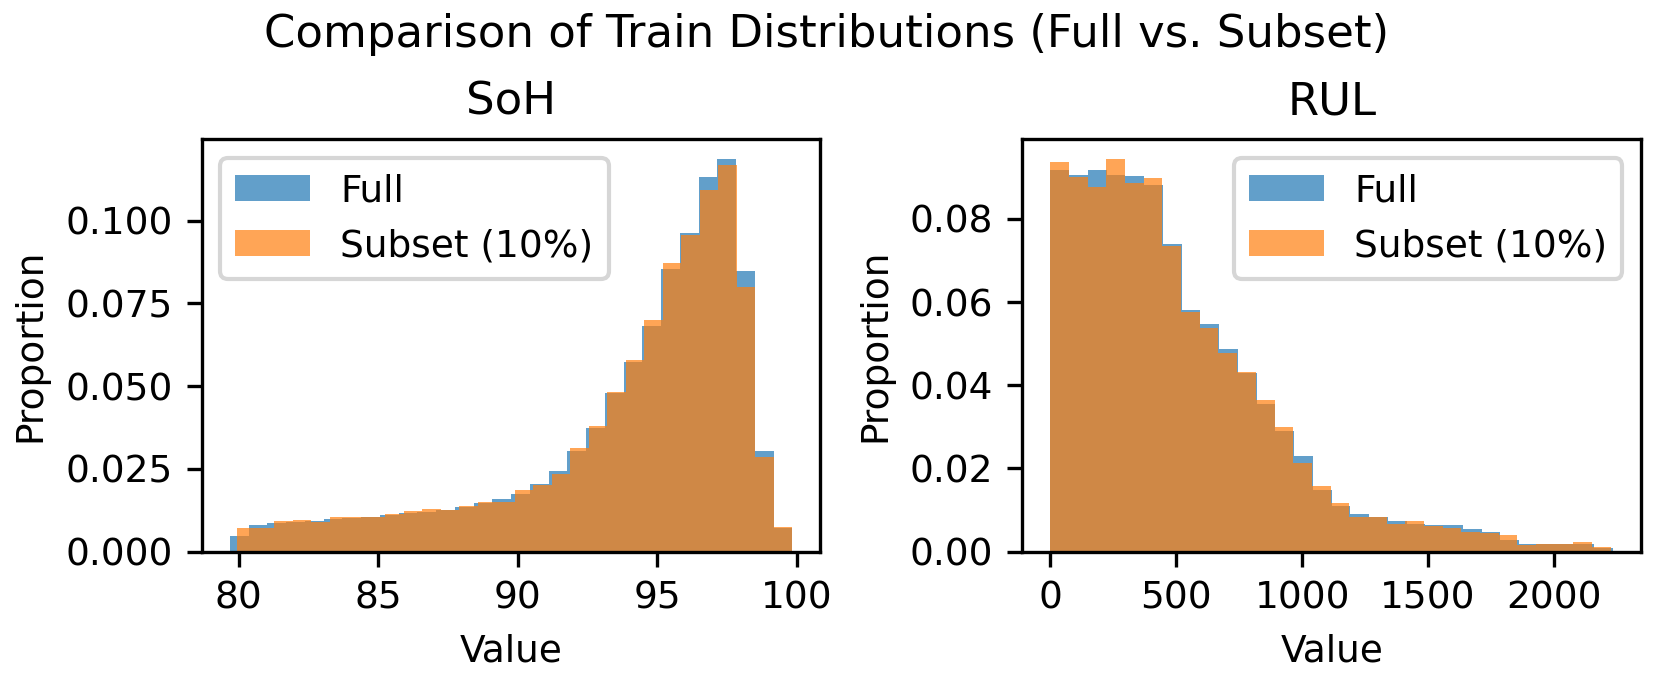
\includegraphics[width=0.8\textwidth]{_img_subset_distributions.png}
    \caption{Distribution of targets on both full train data and subset of 10\% used to hyperparameters optimization.}
    \label{fig:subset_distributions}
\end{figure}


% Summarizing the methodology
This methodology leverages full-life data from training cells to develop models that generalize to unseen cells, addressing the challenges of \ac{soh} and \ac{rul} estimation. Through standardized features, multi-object optimization and hyperparameter optimization via TPE and cross-validation, the approach ensures robust predictions avoiding artificially inflated metrics due to overfitting.

\section{Results} \label{sec:results}

\subsection{Optimization Results \textcolor{red}{and Validation}}

Table \ref{tab:soh_optim} and \ref{tab:rul_optim} below show the results of the optimization process for both \acf{soh} and \acf{rul}, respectively. It can be seen that the models produced good values of validation \acf{rmse}, which is the average of the \ac{rmse} on each fold of cross validation, while maintaining low relative gaps which is a good indicative of non-overfitting models. For \ac{rul} models, authough it was harder to keep the relative gap values low, which indicates models for that target with the features extracted on this work are more prone to overfitt the training data.\todo[size=\tiny]{[R1] Authors should explain how 4 features results in better outcomes than 16, Explain in detail w/ Physics.}

\textcolor{red}{Model selection and evaluation followed a two-stage design: hyperparameter selection was carried out with 5-fold Group K-Fold cross-validation using only training cells (cell-wise separation), and the final selected models were then evaluated on a fully disjoint test set of 25 cells. This ensures that validation scores characterize model-selection performance while test scores quantify cross-cell generalization.}

% Table for SOH
\begin{table}[H]
    \centering
    \caption{Mean training and validation RMSE and relative gap across folds for machine learning models predicting State of Health (SOH) using 4 or 16 features, evaluated via 5-fold cross-validation.}
    \label{tab:soh_optim}
    \begin{tabular}{lcrrr}
    \toprule
    Model & Features & \multicolumn{2}{c}{RMSE} & Relative Gap \\
    \cmidrule(lr){3-4}
          &          & Train & Validation & \\
    \midrule
    \multirow{2}{*}{LGBMRegressor}       & 16 & 0.52 & 0.94 & 0.44 \\
                                         & 4  & 0.86 & 1.22 & 0.29 \\
    \cmidrule{1-5}
    \multirow{2}{*}{ExtraTreesRegressor} & 16 & 0.78 & 1.07 & 0.27 \\
                                         & 4  & 1.23 & 1.40 & 0.12 \\
    \cmidrule{1-5}
    \multirow{2}{*}{KNeighborsRegressor} & 16 & 0.80 & 1.28 & 0.38 \\
                                         & 4  & 1.15 & 1.50 & 0.24 \\
    \cmidrule{1-5}
    \multirow{2}{*}{TweedieRegressor}    & 16 & 1.66 & 1.77 & 0.06 \\
                                         & 4  & 2.03 & 2.06 & 0.01 \\
    \bottomrule
    \end{tabular}
\end{table}

% Table for RUL
\begin{table}[H]
    \centering
    \caption{Mean training and validation RMSE and relative gap across folds for machine learning models predicting Remaining Useful Life (RUL) using 4 or 16 features, evaluated via 5-fold cross-validation.}
    \label{tab:rul_optim}
    \begin{tabular}{lcrrr}
    \toprule
    Model & Features & \multicolumn{2}{c}{RMSE} & Relative Gap \\
    \cmidrule(lr){3-4}
          &          & Train & Validation & \\
    \midrule
    \multirow{2}{*}{ExtraTreesRegressor} & 16 & 31.38 & 103.64 & 0.70 \\
                                         & 4  & 52.33 & 110.00 & 0.52 \\
    \cmidrule{1-5}
    \multirow{2}{*}{LGBMRegressor}       & 16 & 18.51 & 106.14 & 0.83 \\
                                         & 4  & 22.12 & 109.09 & 0.80 \\
    \cmidrule{1-5}
    \multirow{2}{*}{KNeighborsRegressor} & 16 & 56.22 & 143.10 & 0.61 \\
                                         & 4  & 51.19 & 112.09 & 0.54 \\
    \cmidrule{1-5}
    \multirow{2}{*}{TweedieRegressor}    & 16 & 367.01 & 367.01 & 0.00 \\
                                         & 4  & 337.10 & 340.03 & 0.01 \\
    \bottomrule
    \end{tabular}
\end{table}


Tables \ref{tab:soh_hyperparams} and \ref{tab:rul_hyperparams} show the optimimal values of the hyperparams for \ac{soh} and \ac{rul}, respectively. 

\begin{table}[p]
    \centering
    \caption{Optimal hyperparameters for SOH prediction}
    \label{tab:soh_hyperparams}
    \resizebox{0.81\textwidth}{!}{%
    \begin{tabular}{lllc}
    \toprule
    Model & Num. Features & Hyper Param & Optimal Value \\
    \midrule
    \multirow{5}{*}{ExtraTreesRegressor} & \multirow{5}{*}{\num{16}} & n\_estimators & \num{87} \\
    & & max\_depth & \num{7} \\
    & & min\_samples\_split & \num{3} \\
    & & min\_samples\_leaf & \num{1} \\
    & & criterion & squared\_error \\
    \cmidrule(l){2-4}
    & \multirow{5}{*}{\num{4}} & n\_estimators & \num{87} \\
    & & max\_depth & \num{7} \\
    & & min\_samples\_split & \num{3} \\
    & & min\_samples\_leaf & \num{1} \\
    & & criterion & squared\_error \\
    \midrule
    \multirow{3}{*}{KNeighborsRegressor} & \multirow{3}{*}{\num{16}} & n\_neighbors & \num{35} \\
    & & weights & uniform \\
    & & p & \num{1} \\
    \cmidrule(l){2-4}
    & \multirow{3}{*}{\num{4}} & n\_neighbors & \num{35} \\
    & & weights & uniform \\
    & & p & \num{1} \\
    \midrule
    \multirow{9}{*}{LGBMRegressor} & \multirow{9}{*}{\num{16}} & n\_estimators & \num{661} \\
    & & learning\_rate & \num{0.0066019849581648} \\
    & & num\_leaves & \num{18} \\
    & & max\_depth & \num{5} \\
    & & min\_child\_samples & \num{13} \\
    & & subsample & \num{0.864803089169032} \\
    & & colsample\_bytree & \num{0.8187787356776066} \\
    & & reg\_alpha & \num{0.1252281430305362} \\
    & & reg\_lambda & \num{0.00005994036749692399} \\
    \cmidrule(l){2-4}
    & \multirow{9}{*}{\num{4}} & n\_estimators & \num{661} \\
    & & learning\_rate & \num{0.0066019849581648} \\
    & & num\_leaves & \num{18} \\
    & & max\_depth & \num{5} \\
    & & min\_child\_samples & \num{13} \\
    & & subsample & \num{0.864803089169032} \\
    & & colsample\_bytree & \num{0.8187787356776066} \\
    & & reg\_alpha & \num{0.1252281430305362} \\
    & & reg\_lambda & \num{0.00005994036749692399} \\
    \midrule
    \multirow{4}{*}{TweedieRegressor} & \multirow{4}{*}{\num{16}} & power & \num{1.3779972601681014} \\
    & & alpha & \num{0.00001951722464144947} \\
    & & fit\_intercept & True \\
    & & tol & \num{0.0001331121608073} \\
    \cmidrule(l){2-4}
    & \multirow{4}{*}{\num{4}} & power & \num{1.3779972601681014} \\
    & & alpha & \num{0.00001951722464144947} \\
    & & fit\_intercept & True \\
    & & tol & \num{0.0001331121608073} \\
    \bottomrule
    \end{tabular}
    }
\end{table}

\begin{table}[p]
    \centering
    \caption{Optimal hyperparameters for RUL prediction}
    \label{tab:rul_hyperparams}
    \resizebox{0.81\textwidth}{!}{%
    \begin{tabular}{lllc}
    \toprule
    Model & Num. Features & Hyper Param & Optimal Value \\
    \midrule
    \multirow{5}{*}{ExtraTreesRegressor} & \multirow{5}{*}{\num{16}} & n\_estimators & \num{62} \\
    & & max\_depth & \num{10} \\
    & & min\_samples\_split & \num{4} \\
    & & min\_samples\_leaf & \num{4} \\
    & & criterion & squared\_error \\
    \cmidrule(l){2-4}
    & \multirow{5}{*}{\num{4}} & n\_estimators & \num{110} \\
    & & max\_depth & \num{10} \\
    & & min\_samples\_split & \num{9} \\
    & & min\_samples\_leaf & \num{2} \\
    & & criterion & squared\_error \\
    \midrule
    \multirow{3}{*}{KNeighborsRegressor} & \multirow{3}{*}{\num{16}} & n\_neighbors & \num{35} \\
    & & weights & uniform \\
    & & p & \num{1} \\
    \cmidrule(l){2-4}
    & \multirow{3}{*}{\num{4}} & n\_neighbors & \num{21} \\
    & & weights & uniform \\
    & & p & \num{2} \\
    \midrule
    \multirow{9}{*}{LGBMRegressor} & \multirow{9}{*}{\num{16}} & n\_estimators & \num{563} \\
    & & learning\_rate & \num{0.0293415275650007} \\
    & & num\_leaves & \num{17} \\
    & & max\_depth & \num{7} \\
    & & min\_child\_samples & \num{9} \\
    & & subsample & \num{0.5325257964926398} \\
    & & colsample\_bytree & \num{0.9744427686266666} \\
    & & reg\_alpha & \num{0.530953226900921} \\
    & & reg\_lambda & \num{0.0293210004718329} \\
    \cmidrule(l){2-4}
    & \multirow{9}{*}{\num{4}} & n\_estimators & \num{400} \\
    & & learning\_rate & \num{0.1123189435432641} \\
    & & num\_leaves & \num{24} \\
    & & max\_depth & \num{9} \\
    & & min\_child\_samples & \num{15} \\
    & & subsample & \num{0.7774469727501079} \\
    & & colsample\_bytree & \num{0.6752997137819545} \\
    & & reg\_alpha & \num{0.000574402723477} \\
    & & reg\_lambda & \num{0.0000355834220233792} \\
    \midrule
    \multirow{4}{*}{TweedieRegressor} & \multirow{4}{*}{\num{16}} & power & \num{1.3779972601681014} \\
    & & alpha & \num{0.00001951722464144947} \\
    & & fit\_intercept & True \\
    & & tol & \num{0.0001331121608073} \\
    \cmidrule(l){2-4}
    & \multirow{4}{*}{\num{4}} & power & \num{1.7609371175115585} \\
    & & alpha & \num{0.00002769889922756281} \\
    & & fit\_intercept & True \\
    & & tol & \num{0.000009462175356461489} \\
    \bottomrule
    \end{tabular}
    }
\end{table}

\subsection{Test Results}

The results of each model type using the optimal hyperparam set are shown on \cref{tab:soh_metrics,tab:rul_metrics} for \ac{soh} and \ac{rul}, respectively. The performance drop between using 16 and 4 features were relatively low indicating models with only the most important features identifies by the Tree-based ensamble described in Section \ref{sec:feature_extraction} is feasible.

The overall performance of all models is satisfactory with \ac{rmse} values below 0.80\% for \ac{soh} using a LGBMRegressor for 75\% of the test cells and below 59.91 for \ac{rul} using an ExtraTreesRegressor for 75\% of the test cells. \ac{r2} values for 75\% of the test cells were above 0.97 and 0.96 for \ac{soh} and \ac{rul}, respectively. Indicating high accordance between the models estimations and references values.

% Table for SOH
\begin{table}[H]
    \centering
    \caption{Performance metrics (RMSE and R²) for machine learning models predicting State of Health (SOH) using 4 or 16 features, evaluated via 5-fold cross-validation.}
    \label{tab:soh_metrics}
    \begin{tabular}{lcrrrr}
    \toprule
    Model & Features & \multicolumn{2}{c}{RMSE} & \multicolumn{2}{c}{R²} \\
    \cmidrule(lr){3-4} \cmidrule(lr){5-6}
          &          & Median & Q3 & Median & Q1 \\
    \midrule
    \multirow{2}{*}{LGBMRegressor}       & 16 & 0.71 & 0.80 & 0.97 & 0.96 \\
                                         & 4  & 0.96 & 1.25 & 0.95 & 0.90 \\
    \cmidrule{1-6}
    \multirow{2}{*}{KNeighborsRegressor} & 16 & 0.69 & 1.14 & 0.98 & 0.90 \\
                                         & 4  & 1.04 & 1.32 & 0.94 & 0.88 \\
    \cmidrule{1-6}
    \multirow{2}{*}{ExtraTreesRegressor} & 16 & 0.83 & 0.97 & 0.97 & 0.94 \\
                                         & 4  & 0.96 & 1.32 & 0.95 & 0.89 \\
    \cmidrule{1-6}
    \multirow{2}{*}{TweedieRegressor}    & 16 & 1.36 & 2.33 & 0.88 & 0.70 \\
                                         & 4  & 1.63 & 2.24 & 0.81 & 0.70 \\
    \bottomrule
    \end{tabular}
\end{table}

% Table for RUL
\begin{table}[H]
    \centering
    \caption{Performance metrics (RMSE and R²) for machine learning models predicting Remaining Useful Life (RUL) using 4 or 16 features, evaluated via 5-fold cross-validation.}
    \label{tab:rul_metrics}
    \begin{tabular}{lcrrrr}
    \toprule
    Model & Features & \multicolumn{2}{c}{RMSE} & \multicolumn{2}{c}{R²} \\
    \cmidrule(lr){3-4} \cmidrule(lr){5-6}
          &          & Median & Q3 & Median & Q1 \\
    \midrule
    \multirow{2}{*}{ExtraTreesRegressor} & 16 & 41.63 & 59.91 & 0.96 & 0.90 \\
                                         & 4  & 45.21 & 68.41 & 0.96 & 0.91 \\
    \cmidrule{1-6}
    \multirow{2}{*}{LGBMRegressor}       & 16 & 49.46 & 76.74 & 0.95 & 0.89 \\
                                         & 4  & 59.92 & 69.59 & 0.93 & 0.91 \\
    \cmidrule{1-6}
    \multirow{2}{*}{KNeighborsRegressor} & 16 & 54.17 & 95.94 & 0.93 & 0.79 \\
                                         & 4  & 63.85 & 100.44 & 0.91 & 0.81 \\
    \cmidrule{1-6}
    \multirow{2}{*}{TweedieRegressor}    & 16 & 63.52 & 102.68 & 0.90 & 0.71 \\
                                         & 4  & 89.41 & 124.98 & 0.85 & 0.60 \\
    \bottomrule
    \end{tabular}
\end{table}

Figures \ref{fig:best_16_soh_model} to \ref{fig:best_4_rul_model} show in detail the scatter plots of all reference vs. estimated values of all test cells for the best model in each case: \ac{soh} and \ac{rul} and using all 16 features and only 4 features. It can be confirmed that the model works really well for most data while some points are more distant from the ideal fit line. For \ac{soh} models under and over estimate values while for \ac{rul} models tend to under estimate the values. For the \ac{rul} models with 16 and 4 features it can be noticed that a similar set of points diverge from the ideal regression line, we identified that this points correspond to the same cell of the test set. From the plot it can be seen that this cell is the only with almost 2000 cycles cyclelife, this divergence of the model might be happening because data with \ac{rul} values that high are more scarce on the training set as well due to the fact few cells cycle that long on the dataset used.

\begin{figure}[H]
    \centering
    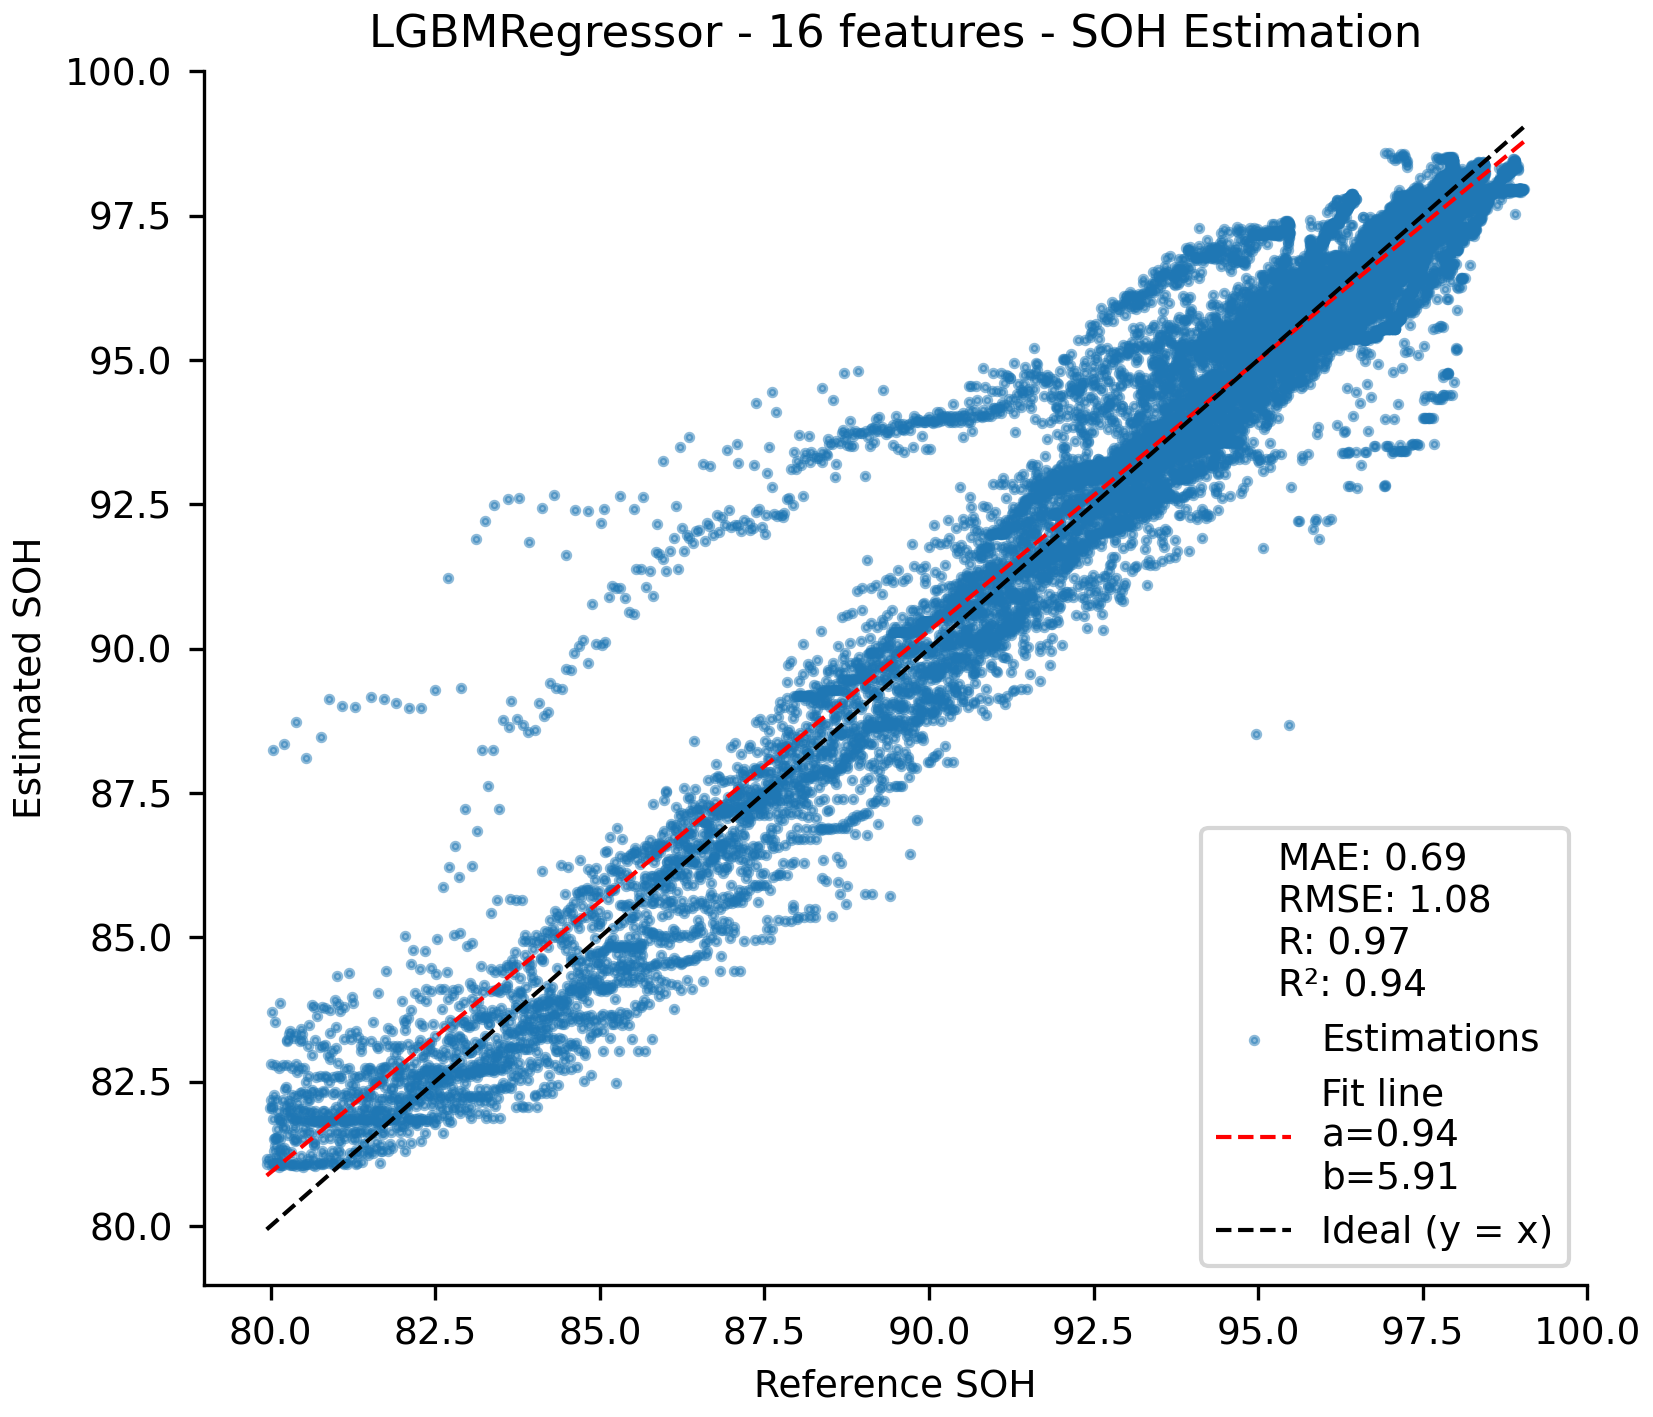
\includegraphics[width=0.8\textwidth]{_img_16_features_LGBMRegressor_SOH_scatter.png}
    \caption{Predicted vs. true \ac{soh} for test cells using 16 features. The dashed line shows the ideal $y=x$ fit. Performance metrics (\ac{rmse}, \ac{mae}, \ac{r2}) are reported per panel.}
    \label{fig:best_16_soh_model}
\end{figure}

\begin{figure}[H]
    \centering
    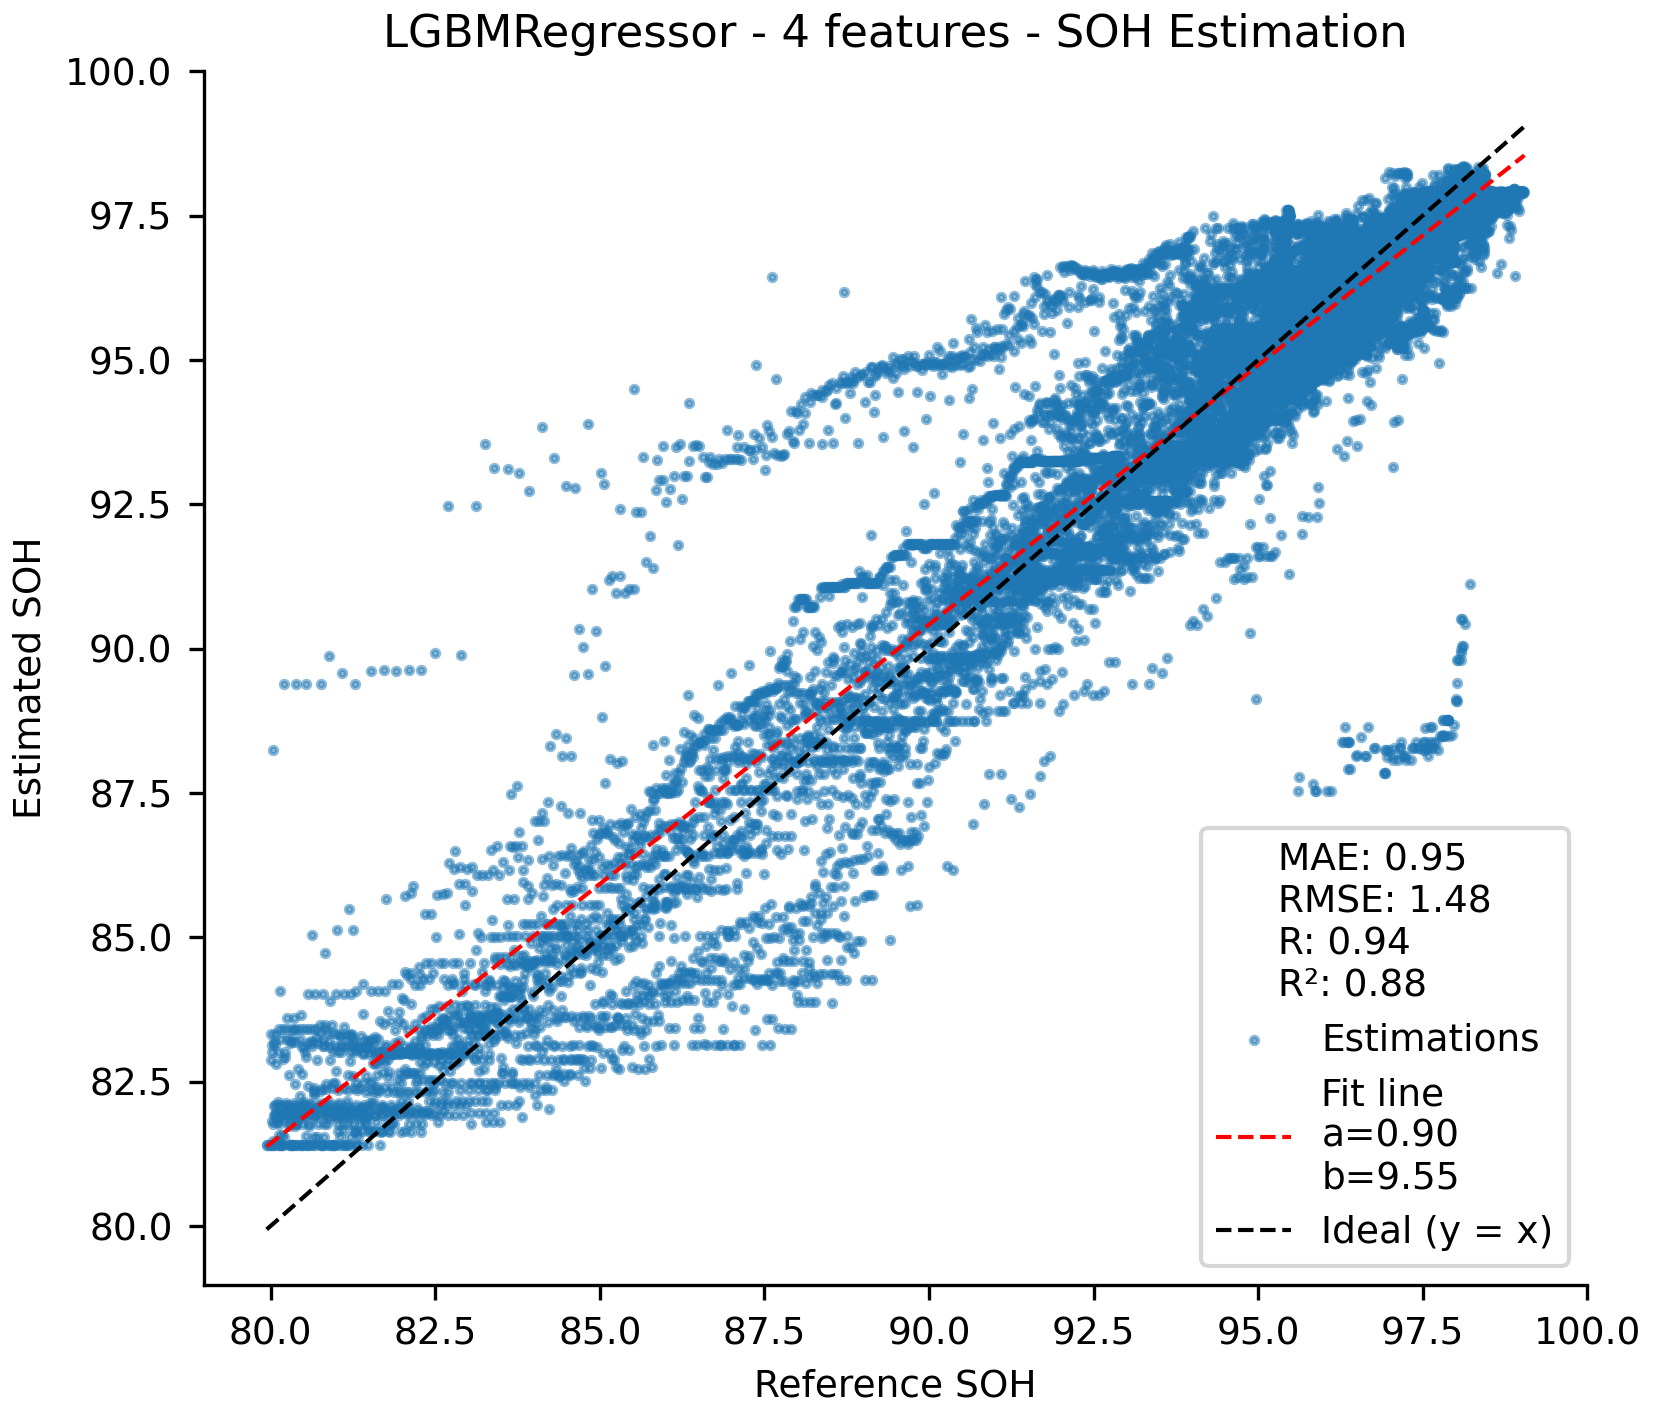
\includegraphics[width=0.8\textwidth]{_img_4_features_LGBMRegressor_SOH_scatter.png}
    \caption{Predicted vs. true \ac{soh} for test cells using four features. The dashed line shows the ideal $y=x$ fit. Performance metrics (\ac{rmse}, \ac{mae}, \ac{r2}) are reported per panel.}
    \label{fig:best_4_soh_model}
\end{figure}

\begin{figure}[H]
    \centering
    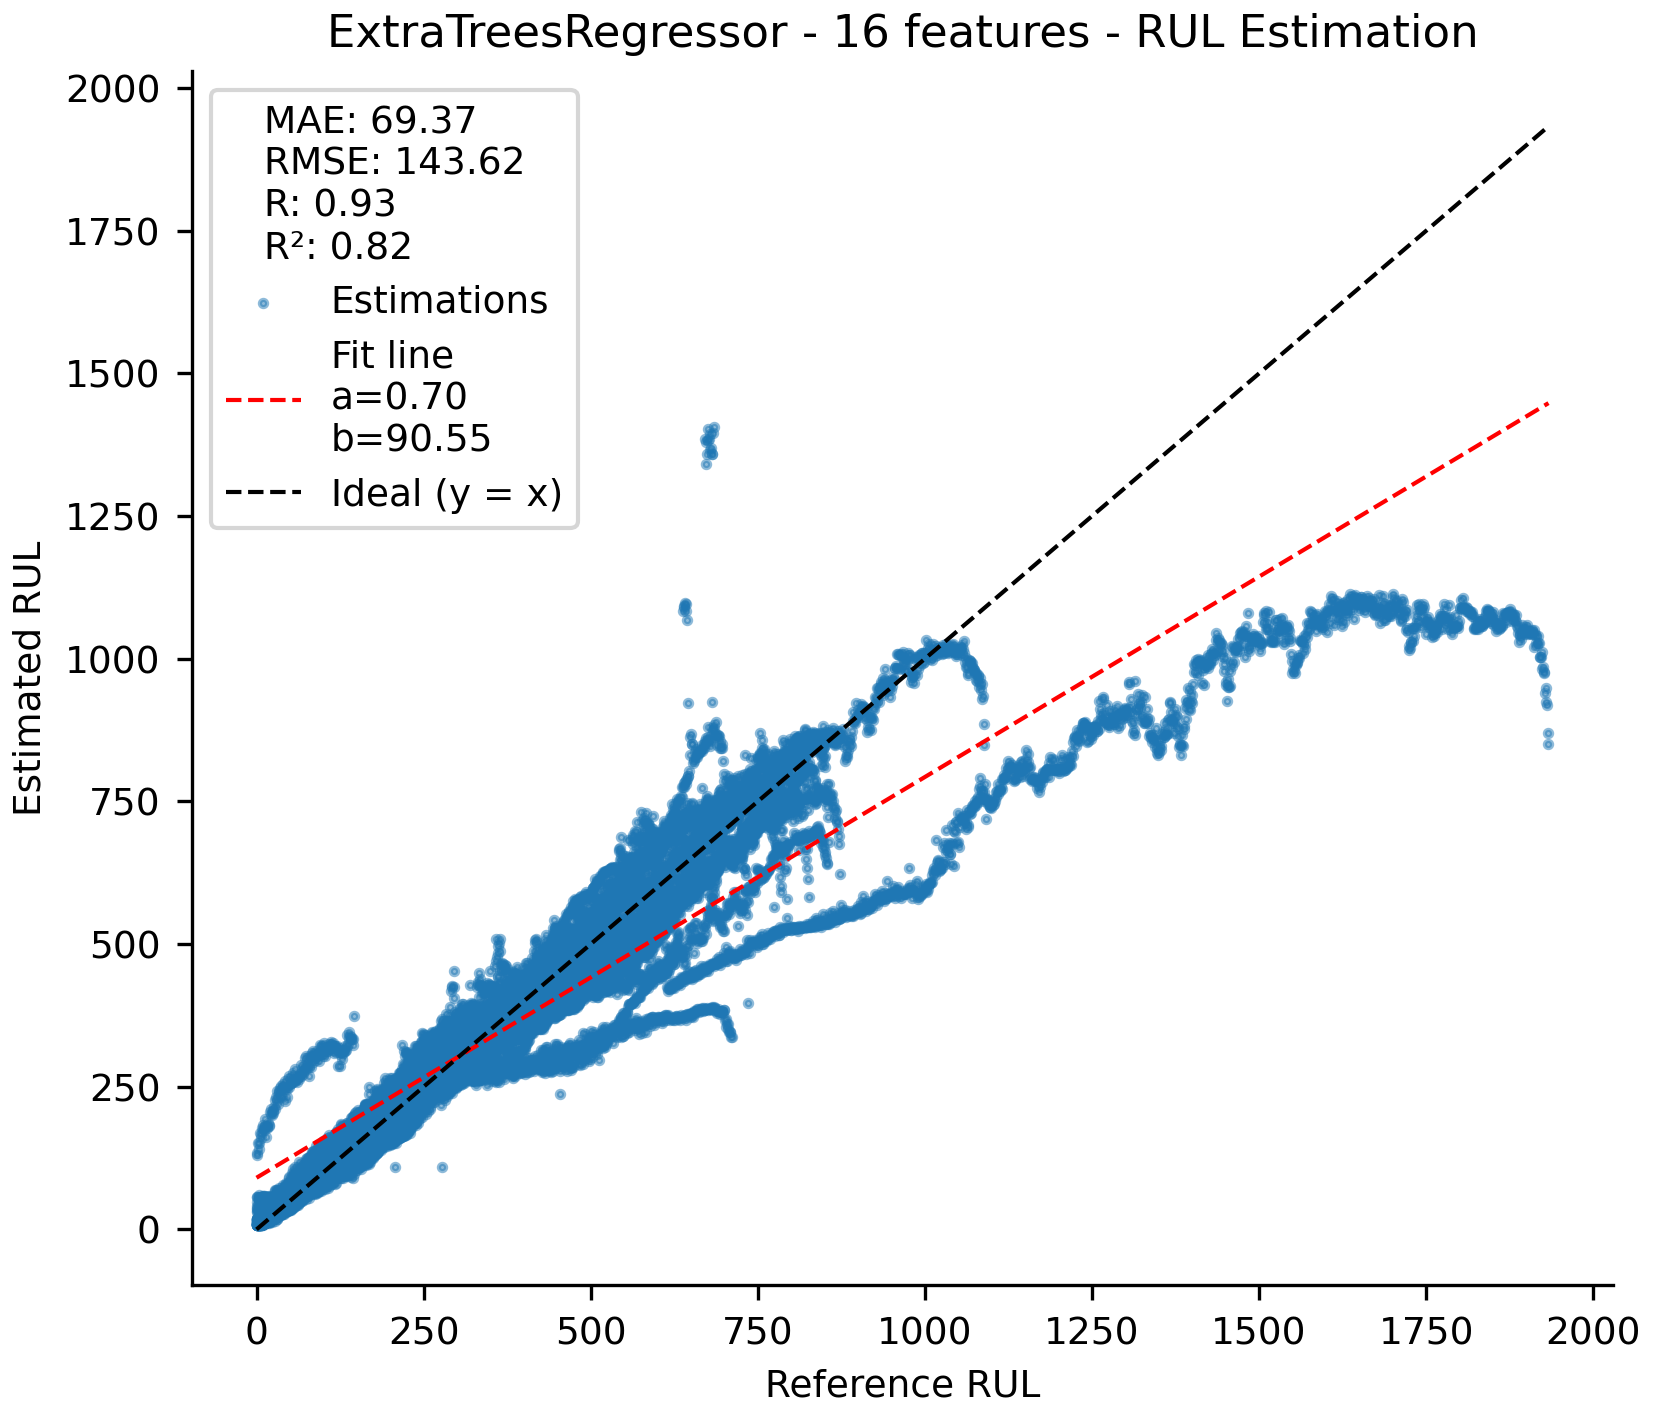
\includegraphics[width=0.8\textwidth]{_img_16_features_ExtraTreesRegressor_RUL_scatter.png}
    \caption{Predicted vs. true \ac{rul} for test cells using 16 features. The dashed line shows the ideal $y=x$ fit. Performance metrics (\ac{rmse}, \ac{mae}, \ac{r2}) are reported per panel.}
    \label{fig:best_16_rul_model}
\end{figure}

\begin{figure}[H]
    \centering
    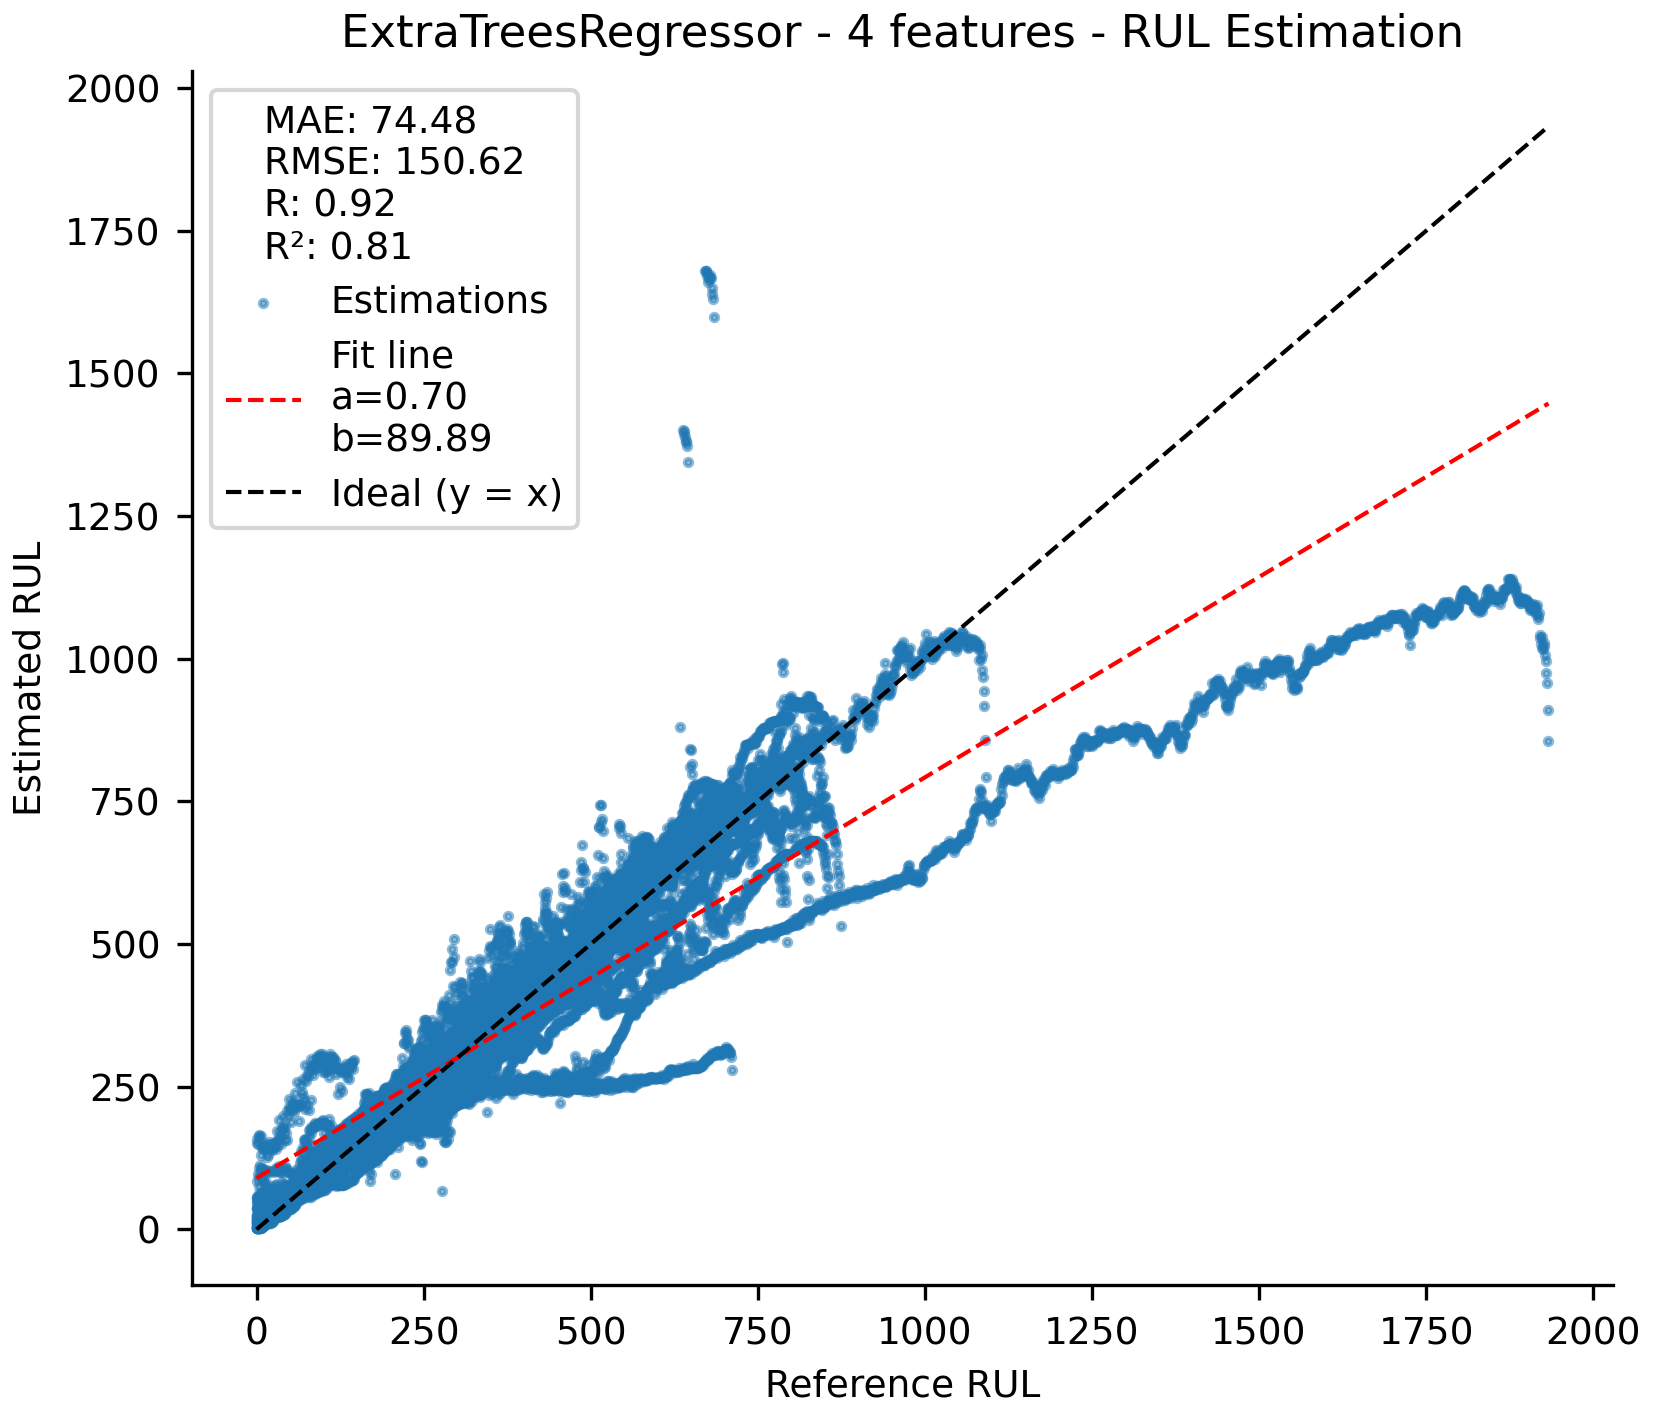
\includegraphics[width=0.8\textwidth]{_img_4_features_ExtraTreesRegressor_RUL_scatter.png}
    \caption{Predicted vs. true \ac{rul} for test cells using four features. The dashed line shows the ideal $y=x$ fit. Performance metrics (\ac{rmse}, \ac{mae}, \ac{r2}) are reported per panel.}
    \label{fig:best_4_rul_model}
\end{figure} \todo[size=\tiny]{[R2] Prediction deviation is large for cells with long timestamp. Explain whether the characteristics of these abnormal cells, such as charging protocols and temperatures anomalies, have been analyzed.}






\section{Results and Discussion}
\subsection{Hyperparameter Optimization Performance}
The hyperparameter optimization process successfully identified optimal configurations for all machine learning models across both \ac{soh} and \ac{rul} prediction tasks. Tables \ref{tab:soh_optim} and \ref{tab:rul_optim} present the cross-validation performance metrics obtained during the optimization phase, revealing distinct patterns in model behavior and generalization capabilities.

For \ac{soh} prediction (Table \ref{tab:soh_optim}), the LGBMRegressor demonstrated superior performance with the lowest validation \ac{rmse} of 0.94\% when utilizing all 16 features, while maintaining a moderate relative gap of 0.44. This indicates a balanced trade-off between predictive accuracy and overfitting resistance. The ExtraTreesRegressor achieved comparable performance with a validation \ac{rmse} of 1.07\% and notably lower relative gap of 0.27, suggesting better generalization properties. The TweedieRegressor, while exhibiting excellent generalization characteristics ($relative gaps \leq 0.06$), showed substantially higher validation errors, indicating insufficient model complexity for capturing the underlying \ac{soh} patterns.

\ac{rul} prediction (Table \ref{tab:rul_optim}) proved more challenging, with all models exhibiting higher relative gaps compared to \ac{soh} estimation, suggesting increased susceptibility to overfitting. The ExtraTreesRegressor achieved the best validation performance with an \ac{rmse} of 103.64 cycles using 16 features, though with a concerning relative gap of 0.70. The LGBMRegressor, despite lower training error (18.51 cycles), showed an even larger relative gap of 0.83, indicating significant overfitting tendencies. The TweedieRegressor again demonstrated perfect generalization ($relative gap \approx 0.00$) but at the cost of substantially higher prediction errors.\todo[size=\tiny]{[R1] How to find cycle errors in SOH and RUL prediction. Confirm if these errors are significant in EV applications.}

\subsection{Impact of Feature Reduction}
The transition from 16 to 4 features resulted in predictable but manageable performance degradation across all models. For \ac{soh} prediction, validation \ac{rmse} increased by 20--30\% for tree-based methods (LGBMRegressor: $0.94\% \rightarrow 1.22\%$, ExtraTreesRegressor: $1.07\% \rightarrow
1.40\%$), while simultaneously reducing overfitting tendencies as evidenced by decreased relative gaps. This trade-off suggests that the four most important features capture the majority of \ac{soh}-relevant information, with additional features contributing primarily to model complexity rather than fundamental predictive power.

The feature reduction impact on \ac{rul} prediction was less pronounced, with validation \ac{rmse} changes typically within 10\% (ExtraTreesRegressor: $103.64 \rightarrow 110.00$ cycles). Notably, the reduced feature set generally improved generalization capabilities, with several models showing decreased relative gaps. This pattern indicates that \ac{rul} prediction may be more robust to feature dimensionality reduction, possibly due to the inherent noise in cycle-life estimation making additional features less beneficial.

\subsection{Optimal Hyperparameter Analysis}
The optimal hyperparameters (Table \ref{tab:soh_hyperparams} and \ref{tab:rul_hyperparams}) reveal consistent patterns that provide insights into the underlying data characteristics and model requirements. For tree-based methods, the optimal configurations favored relatively shallow trees ($max\_depth \leq 10$) and small leaf sizes ($min\_samples\_leaf \leq 4$), suggesting that the battery aging patterns can be captured without excessive model complexity. The LGBMRegressor consistently selected low learning rates (0.007--0.11) paired with moderate numbers of estimators (400--661), indicating a preference for gradual learning to avoid overfitting.

Interestingly, the KNeighborsRegressor optimal configurations showed preference for relatively large neighborhood sizes (n\_neighbors = 21--35) and uniform weighting, suggesting that local averaging over substantial regions of the feature space is beneficial for battery prognostics. The consistent selection of Manhattan distance (p=1p=1
p=1) over Euclidean distance (p=2p=2
p=2) for most configurations may indicate that the standardized features exhibit more meaningful relationships under L1 norm.

\subsection{Model-Specific Performance Characteristics}

The superior performance of tree-based ensemble methods (LGBMRegressor and ExtraTreesRegressor) aligns with their inherent ability to capture non-linear relationships and feature interactions without explicit modeling. Battery aging involves complex, non-linear degradation mechanisms that these methods can naturally accommodate. The gradient boosting approach of LGBMRegressor appears particularly well-suited for \ac{soh} estimation, where sequential refinement of predictions can effectively model the gradual capacity fade patterns.
The consistently poor performance of TweedieRegressor, despite its excellent generalization properties, suggests that linear models---even with flexible error distributions---are insufficient for capturing the complexity of battery degradation patterns encoded in the extracted features. This finding reinforces the necessity of non-linear modeling approaches for battery prognostics applications.

\subsection{Test Set Performance and Model Validation}

The test set results (Tables \ref{tab:soh_metrics} and \ref{tab:rul_metrics}) demonstrate that the optimized models successfully generalize to unseen cells, with performance metrics closely matching the cross-validation estimates. For \ac{soh} prediction, the LGBMRegressor achieved an \ac{rmse} below 0.80\% for 75\% of test cells, with \acf{r2} values above 0.97, indicating high accordance between model estimations and reference values. Similarly, for \ac{rul} prediction, the ExtraTreesRegressor maintained \ac{rmse} values below 59.91 cycles for 75\% of test cells, with \ac{r2} values above 0.96.
The scatter plots (Figures \ref{fig:best_16_soh_model} through to \ref{fig:best_4_rul_model}) provide detailed visualization of model performance across all test samples. For \ac{soh} models, the predictions show balanced distribution around the ideal fit line, with both under- and over-estimation patterns. In contrast, \ac{rul} models exhibit a tendency toward under-estimation, particularly evident in the high-cycle region where one test cell with approximately 2000 cycles consistently deviates from the ideal regression line. This divergence likely stems from the scarcity of such long-lived cells in the training dataset, highlighting a limitation in model generalization to extreme cycle-life scenarios.

\subsection{Practical Implications and Deployment Considerations}

From a practical battery management perspective, the results demonstrate that effective \ac{soh} and \ac{rul} estimation can be achieved using a minimal feature set derived from single charge-discharge cycles sampled at 1~Hz or higher. The 4-feature models, while showing modest performance reduction, offer significant computational advantages for embedded applications where processing power and memory are constrained.

However, a critical limitation for real-world deployment concerns data availability. The feature extraction methodology requires complete constant current constant voltage (CCCV) charge-discharge cycle data, which may not be readily available during normal battery operation in applications such as electric vehicles or grid energy storage systems. Such complete cycling data would typically only be obtainable during dedicated diagnostic procedures with the load disconnected from the battery, limiting the frequency of prognostic updates and potentially compromising the timeliness of health assessments. This constraint necessitates careful consideration of diagnostic scheduling and may require development of alternative feature extraction methods that can operate on partial cycle data or operational load profiles.

Despite this limitation, the observed performance characteristics suggest different deployment strategies for \ac{soh} and \ac{rul} estimation. \ac{soh} models demonstrate robust performance across the full range of battery conditions, making them suitable for periodic diagnostic monitoring applications. \ac{rul} models, while showing excellent performance for typical battery lifespans, may require additional training data or specialized handling for batteries exhibiting exceptional longevity, and their deployment would be similarly constrained by the need for complete cycle data.

\subsection{Limitations and Future Research Directions}

Several limitations must be acknowledged in the current optimization approach. The use of a 10\% subset (Figure \ref{fig:subset_distributions}) for hyperparameter optimization, while computationally efficient, may not fully capture the complete data distribution complexity.\todo[size=\tiny]{[R2] Does this imply the optimizatin results might unstable?} Additionally, the focus on full-life training data, while comprehensive for model evaluation, may not reflect real-world scenarios where models must perform early-life predictions with limited degradation history.

A fundamental limitation lies in the requirement for complete CCCV cycle data for feature extraction. This dependency significantly restricts the practical applicability of the developed models, as such data is typically unavailable during normal battery operation and can only be obtained during scheduled diagnostic procedures. Future research should prioritize the development of feature extraction methods that can operate on partial cycle data, operational load profiles, or other readily available signals to enable continuous prognostic monitoring without service interruption.

The identified overfitting tendencies, particularly for \ac{rul} prediction, highlight the need for regularization strategies beyond hyperparameter optimization. Future work should investigate ensemble approaches that combine multiple models or incorporate physics-informed constraints to improve generalization while maintaining predictive accuracy. The development of hybrid models that combine the generalization properties of simpler methods with the predictive power of complex ensemble approaches could address the observed overfitting issues.

The consistent challenges observed in \ac{rul} prediction across all models indicate a need for alternative problem formulations, such as classification-based approaches that predict remaining life ranges rather than precise cycle counts, or multi-task learning frameworks that jointly optimize \ac{soh} and \ac{rul} estimation to leverage their inherent relationships. Additionally, investigating domain-specific regularization techniques that incorporate known battery aging physics could improve model robustness and reduce the sensitivity to training data distribution variations.

\input{__sec09_conclusion}
\input{__sec10_appendix}


\section*{CRediT author statement}
\textbf{Gabriel Buzzi Sanches}: Conceptualization, Methodology, Software, Writing – original draft; \textbf{Carlos Antonio Rufino Jr}: Conceptualization, Methodology, Software, Supervision, Writing – original draft, Writing – review \& editing; \textbf{Lucas Saraiva Teixeira}: Writing – review \& editing; \textbf{Hans-Georg Schweiger}: Funding acquisition, Project administration, Supervision, Writing – review \& editing; \textbf{Hudson Giovani Zanin}: Funding acquisition, Project administration, Resources, Supervision, Writing – review \& editing


\section*{Acknowledgments}
C.A.R.J. and H.Z. would like to thank CNPq (159332/2019-2), who have provided financial support. H.Z. would like to thank the National Council for Scientific and Technological Development (CNPq, Brazil) (301486/2016-6), São Paulo State Research Support Foundation (FAPESP, Brazil) (2014/02163-7, 2017/11958-1, 2018/20756-6) which help fund this research. H.Z. would additionally like to thank the TotalEnergies SE company who funded part of this research through ANP (Brazil’s National Oil, Natural Gas, and Biofuels Agency). We acknowledge and are grateful for the support by the Open Access Publication Fund from Technische Hochschule Ingolstadt (THI).

\section*{Declaration of Interests}
G.B.S, C.A.R.J, and H.G.Z. have the patent {BR512024003266-5}, which has been licensed to Total Energies SE.

\printacronyms[name=List of Acronyms]


\bibliographystyle{elsarticle-num.bst}
\bibliography{___references}

\end{document}
